\documentclass[11pt,letterpaper]{article}
\pdfminorversion=6
\usepackage[letterpaper,margin=1in]{geometry}
\usepackage[T1]{fontenc}
\usepackage[utf8]{inputenc}
\usepackage{lmodern,microtype}
\usepackage{amsmath,amssymb,mathtools,amsthm}
\usepackage{bm}
\usepackage[normalem]{ulem}
\usepackage{xcolor,graphicx,enumitem,dsfont,tikz}
\usetikzlibrary{arrows.meta,calc}

\usepackage[titles]{tocloft}
\renewcommand{\cftsecleader}{\cftdotfill{\cftdotsep}}
\renewcommand{\cftdotsep}{2}
\setlength{\cftbeforesecskip}{6pt}

\usepackage{hyperref}
\hypersetup{
  colorlinks=true,
  linkcolor=blue!60!black,
  citecolor=green!40!black,
  urlcolor=blue!70!black,
  linktoc=all,
  bookmarksdepth=2,
  pdftitle={The limit shape of uniform random antichains in [0,1] to the power d},
  pdfsubject={Limit shapes, permutation limits, and applications to coordinate orders}
}

\usepackage[nameinlink,capitalize,noabbrev]{cleveref}
\crefname{section}{Section}{Sections}
\Crefname{section}{Section}{Sections}
\crefname{subsection}{Section}{Sections}
\Crefname{subsection}{Section}{Sections}
\crefname{subsubsection}{Section}{Sections}
\Crefname{subsubsection}{Section}{Sections}
\renewcommand*{\sectionautorefname}{Section}
\renewcommand*{\subsectionautorefname}{Section}
\renewcommand*{\subsubsectionautorefname}{Section}

\usepackage[
  backend=biber,
  style=alphabetic,
  maxalphanames=3,
  maxnames=8,
  maxbibnames=20,
  giveninits=true
]{biblatex}
\renewcommand*{\multicitedelim}{\addcomma\space}
\addbibresource{references.bib}
\setlength{\bibitemsep}{2pt}
\AtBeginBibliography{\small\sloppy}

\setlength{\parskip}{3pt}
\setlength{\emergencystretch}{2em}
\setcounter{tocdepth}{2}
\setcounter{secnumdepth}{3}

\numberwithin{equation}{section}
\newtheorem{theorem}{Theorem}[section]

\newtheorem{proposition}[theorem]{Proposition}
\newtheorem{lemma}[theorem]{Lemma}
\newtheorem{corollary}[theorem]{Corollary}
\providecommand*{\propositionautorefname}{Proposition}
\providecommand*{\lemmaautorefname}{Lemma}
\providecommand*{\corollaryautorefname}{Corollary}

\theoremstyle{definition}
\newtheorem{question}[theorem]{Question}
\providecommand*{\questionautorefname}{Question}

\newtheorem{definition}[theorem]{Definition}
\newtheorem{conjecture}[theorem]{Conjecture}
\newtheorem{problem}[theorem]{Problem}
\newtheorem{assumption}[theorem]{Assumption}

\theoremstyle{remark}
\newtheorem{remark}[theorem]{Remark}

\crefname{theorem}{Theorem}{Theorems}
\crefname{proposition}{Proposition}{Propositions}
\crefname{lemma}{Lemma}{Lemmas}
\crefname{corollary}{Corollary}{Corollaries}
\crefname{conjecture}{Conjecture}{Conjectures}
\crefname{problem}{Problem}{Problems}
\crefname{question}{Question}{Questions}
\Crefname{question}{Question}{Questions}

\setlist{topsep=3pt,itemsep=2pt,parsep=0pt}




\newcommand{\R}{\mathbb R}
\newcommand{\C}{\mathbb C}
\newcommand{\N}{\mathbb N}
\newcommand{\one}{\mathbf 1}
\newcommand{\eps}{\varepsilon}
\newcommand{\dd}{\,\mathrm d}

\renewcommand{\P}{\mathbb P}
\newcommand{\E}{\mathbb E}
\newcommand{\law}{\operatorname{Law}}
\newcommand{\TV}{\operatorname{TV}}
\newcommand{\NB}{\operatorname{NB}}
\newcommand{\Ext}{\mathsf{Ext}}
\newcommand{\Surv}{\mathsf{Surv}}
\newcommand{\dto}[1][]{\xrightarrow[#1]{\enskip\mathrm d\enskip}}

\renewcommand{\Re}{\operatorname{Re}}
\renewcommand{\Im}{\operatorname{Im}}
\newcommand{\Res}{\operatorname{Res}}
\newcommand{\PV}{\operatorname{PV}}
\newcommand{\supp}{\operatorname{supp}}
\renewcommand{\th}{\vartheta}
\newcommand{\euler}{\bm{\gamma}_{E}}

\DeclareMathOperator{\wt}{wt}
\newcommand{\rv}{v_\partial}
\newcommand{\hgt}{H}
\newcommand{\Dk}[1]{\mathsf D_{#1}}
\newcommand{\Rk}[2]{\mathsf R^{#1}_{#2}}
\newcommand{\tc}{t_{\mathrm c}}
\newcommand{\muA}{\mu_{\mathrm A}}
\newcommand{\CLE}[1]{\mathrm{CLE}_{#1}}
\newcommand{\cm}{\mathbf{c}_{\mathrm M}}
\newcommand{\cl}{\mathbf{c}_{\mathrm L}}
\newcommand{\bQ}{\bm{\beta}_Q}
\newcommand{\bg}{\mathbf g}
\newcommand{\bh}{\mathbf h}

\newcommand{\cA}{\mathcal A}
\newcommand{\cB}{\mathcal B}
\newcommand{\cC}{\mathcal C}
\newcommand{\cD}{\mathcal D}
\newcommand{\cE}{\mathcal E}
\newcommand{\cF}{\mathcal F}
\newcommand{\cG}{\mathcal G}
\newcommand{\cH}{\mathcal H}
\newcommand{\cI}{\mathcal I}
\newcommand{\cJ}{\mathcal J}
\newcommand{\cK}{\mathcal K}
\newcommand{\cL}{\mathcal L}
\newcommand{\cM}{\mathcal M}
\newcommand{\cN}{\mathcal N}
\newcommand{\cO}{\mathcal O}
\newcommand{\cP}{\mathcal P}
\newcommand{\cQ}{\mathcal Q}
\newcommand{\cR}{\mathcal R}
\newcommand{\cS}{\mathcal S}
\newcommand{\cT}{\mathcal T}
\newcommand{\cU}{\mathcal U}
\newcommand{\cV}{\mathcal V}
\newcommand{\cW}{\mathcal W}
\newcommand{\cX}{\mathcal X}
\newcommand{\cY}{\mathcal Y}
\newcommand{\cZ}{\mathcal Z}

\newcommand{\fA}{\mathfrak A}
\newcommand{\fB}{\mathfrak B}
\newcommand{\fC}{\mathfrak C}
\newcommand{\fD}{\mathfrak D}
\newcommand{\fE}{\mathfrak E}
\newcommand{\fF}{\mathfrak F}
\newcommand{\fG}{\mathfrak G}
\newcommand{\fH}{\mathfrak H}
\newcommand{\fI}{\mathfrak I}
\newcommand{\fJ}{\mathfrak J}
\newcommand{\fK}{\mathfrak K}
\newcommand{\fL}{\mathfrak L}
\newcommand{\fM}{\mathfrak M}
\newcommand{\fN}{\mathfrak N}
\newcommand{\fO}{\mathfrak O}
\newcommand{\fP}{\mathfrak P}
\newcommand{\fQ}{\mathfrak Q}
\newcommand{\fR}{\mathfrak R}
\newcommand{\fS}{\mathfrak S}
\newcommand{\fT}{\mathfrak T}
\newcommand{\fU}{\mathfrak U}
\newcommand{\fV}{\mathfrak V}
\newcommand{\fW}{\mathfrak W}
\newcommand{\fX}{\mathfrak X}
\newcommand{\fY}{\mathfrak Y}
\newcommand{\fZ}{\mathfrak Z}

\newcommand{\fa}{\mathfrak a}
\newcommand{\fb}{\mathfrak b}
\newcommand{\fc}{\mathfrak c}
\newcommand{\fd}{\mathfrak d}
\newcommand{\fe}{\mathfrak e}
\newcommand{\ff}{\bm{\mathfrak f}}
\newcommand{\fg}{\mathfrak g}
\newcommand{\fh}{\mathfrak h}
\newcommand{\fri}{\mathfrak i}
\newcommand{\fj}{\mathfrak j}
\newcommand{\fk}{\mathfrak k}
\newcommand{\fl}{\mathfrak l}
\newcommand{\fm}{\mathfrak m}
\newcommand{\fn}{\mathfrak n}
\newcommand{\fo}{\mathfrak o}
\newcommand{\fp}{\mathfrak p}
\newcommand{\fq}{\mathfrak q}
\newcommand{\fr}{\mathfrak r}
\newcommand{\fs}{\mathfrak s}
\newcommand{\ft}{\mathfrak t}
\newcommand{\fu}{\mathfrak u}
\newcommand{\fv}{\mathfrak v}
\newcommand{\fw}{\mathfrak w}
\newcommand{\fx}{\mathfrak x}
\newcommand{\fy}{\mathfrak y}
\newcommand{\fz}{\mathfrak z}

\newcommand{\mref}[1]{\ref*{P-#1}}
\newcommand{\figp}[3]{\begin{figure}[htbp]\centering
    \begin{minipage}{.87\linewidth}\small\itshape\centering
      [Figure placeholder: #1]\end{minipage}\caption{#2}\label{#3}\end{figure}}
\newcommand{\appx}{  \par\bigskip
  \section*{Appendix}  \addcontentsline{toc}{section}{Appendix}  \setcounter{subsection}{0}  \renewcommand{\thesubsection}{\Alph{subsection}}  \renewcommand{\thesubsubsection}{\thesubsection.\arabic{subsubsection}}  \numberwithin{theorem}{subsection}  \numberwithin{equation}{subsection}  \renewcommand{\theHsubsection}{appendix.\Alph{subsection}}  \renewcommand{\theHsubsubsection}{\theHsubsection.\arabic{subsubsection}}  \renewcommand{\theHtheorem}{\theHsubsection.\arabic{theorem}}  \renewcommand{\theHequation}{\theHsubsection.\arabic{equation}}}

\newif\iftdo
  \tdotrue
  \newcommand{\todo}[1]{\iftdo\textcolor{red}{\textbf{[TODO:} #1\textbf{]}}\fi}
  \DeclareRobustCommand{\andrew}[1]{\iftdo{\normalfont\color{magenta!70!black}#1}\fi}
\DeclareRobustCommand{\ewain}[1]{\iftdo{\normalfont\color{green!40!black}#1}\fi}


\DeclareMathOperator{\Var}{Var}
\newcommand{\ind}{\mathds 1}
\newcommand{\vx}{\mathbf x}
\newcommand{\vy}{\mathbf y}
\newcommand{\vz}{\mathbf z}
\newcommand{\vf}{\mathbf f}
\newcommand{\vg}{\mathbf g}
\newcommand{\vh}{\mathbf h}
\newcommand{\ve}{\mathbf e}
\newcommand{\vv}{\mathbf v}
\newcommand{\vu}{\mathbf u}
\newcommand{\vw}{\mathbf w}
\newcommand{\vX}{\mathbf X}
\newcommand{\vY}{\mathbf Y}
\newcommand{\vG}{\mathbf G}
\newcommand{\vF}{\mathbf F}
\newcommand{\vR}{\mathbf R}
\newcommand{\norm}[1]{\lVert#1\rVert}
\newcommand{\ip}[2]{\langle#1,#2\rangle}
\newcommand{\Ldir}[1]{\mathcal L\left\{#1\right\}}
\newcommand{\Vfit}{V_r^{\mathrm{fit}}}
\DeclareMathOperator{\Vol}{vol}
\DeclareMathOperator{\dist}{dist}
\DeclareMathOperator{\diam}{diam}

\DeclareMathOperator{\Proj}{Proj}
\DeclareMathOperator{\Inv}{Inv}
\DeclareMathOperator{\inv}{inv}
\DeclareMathOperator{\LE}{LE}

\usepackage{longtable,xurl,needspace}
\newcommand{\verificationstatus}[2]{\par\Needspace{12\baselineskip}\smallskip{\normalfont\small\color{blue!55!black}\textbf{#2}\enspace\nolinkurl{#1}.}\par\nopagebreak[4]\smallskip\nopagebreak[4]}
\newcommand{\verificationcomparison}[1]{{\normalfont\footnotesize #1}\par\nopagebreak[4]\smallskip}


\title{The limit shape of uniform random antichains in $[0,1]^d$}
\author{Andrew Elvey Price\thanks{CNRS, Université de Tours, Université d'Orléans, IDP, UMR 7013, F-37200 Tours, France.}\and Minjae Park\thanks{Department of Mathematics and Statistics, Auburn University, USA.}}
\date{\today}
\begin{document}
\maketitle

\begin{abstract}
      For each $d\ge2$, we study $n$ independent uniform points in $[0,1]^d$, conditioned to form an antichain: no point is strictly smaller than another in every coordinate. We prove that the point cloud converges in Hausdorff distance to the closure of the hypersurface
      \[
            \mathcal S_d=\left\{\mathbf x\in(0,1)^d: \sum_{i=1}^d\Phi^{-1}(\mathbf x_i)=0\right\}
      \]
      in probability as $n\to\infty$, where $\Phi$ is the standard normal cumulative distribution function. The proof also shows that the antichain probability $a_n$ satisfies $\log a_n=-\frac{n}{d-1}\log n+\beta_d n+o(n)$ for a finite constant $\beta_d$.
      We identify the limiting empirical distribution and hence the limiting permuton of uniform random $d$-dimensional permutations avoiding a single pattern of size $2$.
\end{abstract}

\begin{center}\begin{minipage}{0.93\linewidth}\small
\textbf{Lean verification companion, 20 November 2026.}
The inventory covers 29 numbered proved assertions (including substantive remarks) and 17 separately tracked claims in the prose. Lean verifies 45 without external mathematical inputs. The coordinate-average central limit statement is checked modulo the general iid central limit theorem. Each proved assertion separately records whether the written
argument follows the same method as Lean. Appendix~\ref{sec:lean-full-proofs} gives
optional detailed expositions for selected results.
Open questions, the conjecture and the heuristic remark retain their original status.
Each statement is annotated; Appendix~\ref{sec:lean-status}
records the exact scope and reproducible checks. The original manuscript is preserved separately.
\end{minipage}\end{center}


\begin{figure}[!htbp]
      \centering
      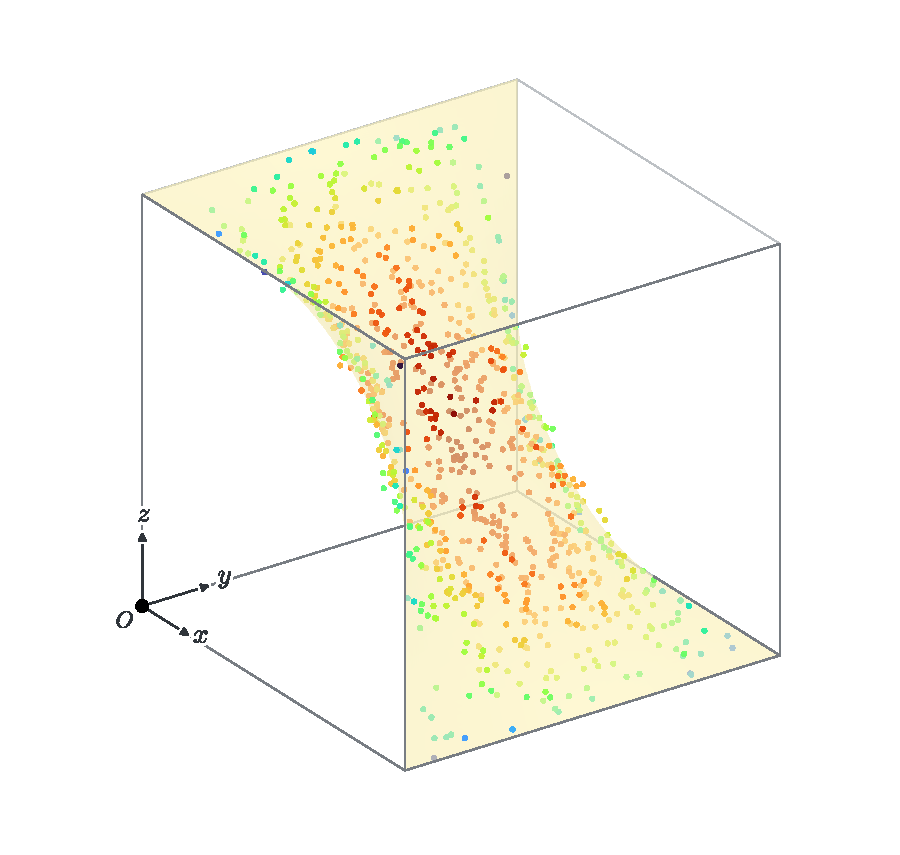
\includegraphics[width=0.47\linewidth]{figures/limit_shape_cube.pdf}\qquad
      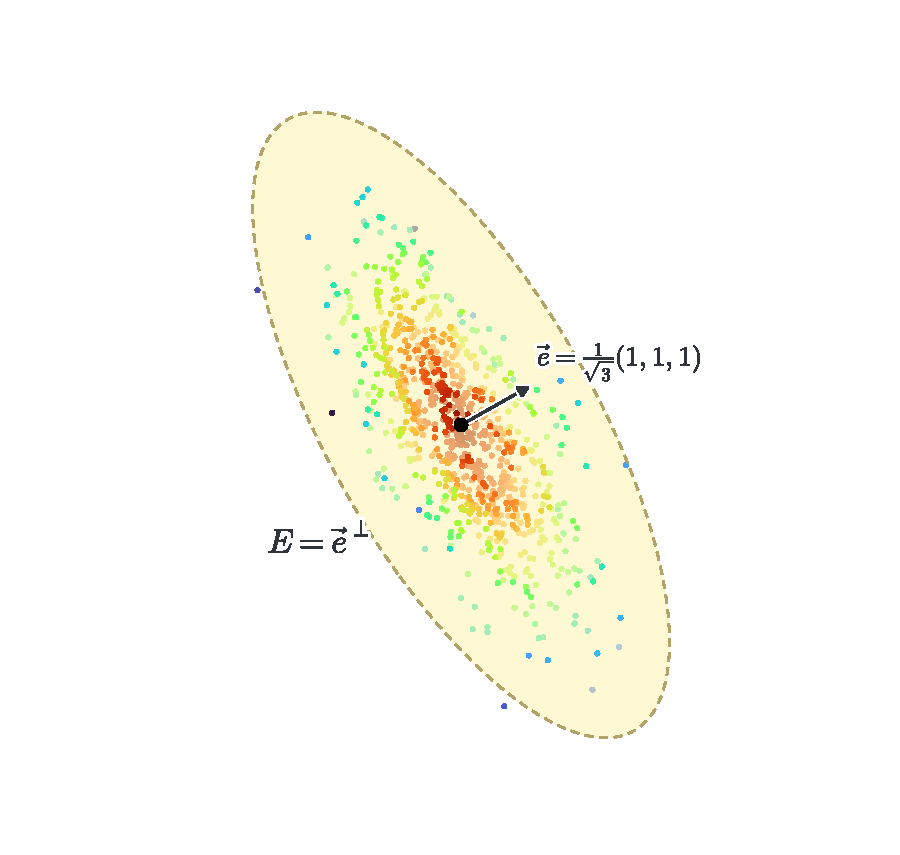
\includegraphics[width=0.47\linewidth]{figures/limit_shape_gaussian.pdf}
      \caption{\textbf{Left:} The surface $\mathcal S_3=\{\mathbf x\in(0,1)^3: \Phi^{-1}(\mathbf x_1)+\Phi^{-1}(\mathbf x_2) +\Phi^{-1}(\mathbf x_3)=0\}$ and a uniform $900$-point antichain sampled by Markov chain Monte Carlo. \textbf{Right:} The same points in Gaussian coordinates $\mathbf g=\Phi^{-1}(\mathbf x)$, with $\Phi^{-1}$ applied coordinatewise, together with a truncated portion of the plane $E=\{\mathbf g\in\R^3: \mathbf g_1+\mathbf g_2+\mathbf g_3=0\}$. Colors indicate $\|\mathbf g\|$ in both coordinate systems.}
      \label{fig:limit-shape}
\end{figure}

\newpage

\tableofcontents

\section{Introduction}

For two points $\vx=(\vx_{1},\ldots,\vx_{d})\in\R^d$ and $\vy=(\vy_{1},\ldots,\vy_{d})\in\R^d$, we write $\vx\prec\vy$ if $\vx_{i}<\vy_{i}$ for each $i\in\{1,\ldots,d\}$. We call a set of points in $\R^d$ an \emph{antichain} if it contains no distinct points $\vx,\vy$ with $\vx\prec\vy$, that is, it is an antichain with respect to the order $\prec$. We study the behavior of uniform random antichains of $n$ points in the cube $[0,1]^d$ as $n\to\infty$. Our main results determine the limit shape of a random antichain and the distribution over this shape. We also improve on previous results regarding the asymptotic form of the probability that $n$ uniform random points form an antichain.

Throughout this paper we fix the dimension $d\ge2$. Let $\vX^{(1)},\ldots,\vX^{(n)}$ be independent uniform points in $[0,1]^d$, and define $\cA_n$ to be the event that these points form an antichain, and $a_{n}$ to be the probability that this occurs:
\[
      \cA_n=\{\vX^{(k)}\not\prec\vX^{(\ell)}\text{ for all }k\ne\ell\}, \qquad a_n=\P(\cA_n).
\]
The first result establishes a linear-order correction to the leading asymptotic of $\log a_n$:

\verificationstatus{ANT-1-1}{Fully Lean-verified}
\verificationcomparison{Statement matches. The draft gives no separate proof; the checked deduction is described below.}
\begin{theorem}\label{thm:counting}
      There is a finite constant $\beta_d$ such that

      \begin{equation}\label{eq:counting}
            \log a_n=-\frac n{d-1}\log n+\beta_d n+o(n).
      \end{equation}
\end{theorem}

\begin{proof}[Proof idea; fully Lean-verified]
Set the weight and height tilt to zero in the proved weighted limit. The actual normal-coordinate change identifies this partition function with the uniform-cube antichain probability. Evaluate the floor Gaussian power integral and absorb its finite contribution into $\beta_d$. Multiplication by $n$ converts the normalized limit into the printed $o(n)$ formula. The underlying weighted proof uses the internally proved alcove geometry.
\end{proof}
As we will discuss, the leading term of this asymptotic was already known. However, the fact that the remaining term, divided by $n$, converges to a finite constant is new for $d\ge3$. The result follows directly from Proposition~\ref{prop:volume}; see Remark~\ref{rem:proof-thm-1}.

Our other results involve the cumulative distribution function $\Phi$ of the standard normal distribution, and its density $\phi$, defined as follows:
\[
      \phi(s)=\frac1{\sqrt{2\pi}}e^{-\frac{s^2}{2}},\qquad \Phi(s)=\int_{-\infty}^s\phi(u)\dd u.
\]
In particular, we show in Theorem~\ref{thm:shape} that uniform random antichains typically approximate the hypersurface
\[
      \cS_d=\left\{\vx\in(0,1)^d:\sum_{i=1}^d\Phi^{-1}(\vx_i)=0\right\}.
\]
Writing $\ve=\frac{1}{\sqrt d}(1,\ldots,1)$ and $E=\ve^\perp$, the limit shape $\cS_d$ can be defined as $\cS_d=\Phi(E)$, where $\Phi$ acts coordinatewise.

To make this statement precise, we define the Hausdorff distance between nonempty compact subsets $A,B\subset[0,1]^d$ by
\[
      d_{\rm H}(A,B)=\max\left\{\sup_{\vx\in A}\dist(\vx,B), \sup_{\vy\in B}\dist(\vy,A)\right\}, \qquad \dist(\vx,B)=\inf_{\vy\in B}\|\vx-\vy\|,
\]
where closures and distances are taken in the closed Euclidean cube $[0,1]^d$.
The Hausdorff distance controls both outliers and holes. Let $A_n=\{\vX^{(1)},\ldots,\vX^{(n)}\}$ denote the uniformly sampled point set and write $\P_n=\P(\,\cdot\mid\cA_n)$ for probability under the uniform antichain model.
The following theorem identifies the shape filled by this set as $\overline{\cS_d}$.
See Figure~\ref{fig:limit-shape} for an illustration when $d=3$.


\verificationstatus{ANT-1-2}{Fully Lean-verified}
\verificationcomparison{Statement matches. The written proof and Lean use the same argument.}
\begin{theorem}\label{thm:shape}
      For every $\delta>0$, there is some $\alpha=\alpha(d,\delta)>0$ such that
      \[
            \P_n\left(d_{\rm H}(A_n,\overline{\cS_d})>\delta \right) \le e^{-\alpha n}
      \]
      for all sufficiently large $n$. In particular, the entire sample fills $\overline{\cS_d}$.
\end{theorem}

\begin{proof}[Proof idea; fully Lean-verified]
Every point in the limiting support has positive mass in each neighborhood, so finitely many continuous tests detect any fixed-size hole. Each point outside the surface closure has a strictly comparable support witness; finitely many such witness tests exclude all distant outliers from an antichain. Apply the empirical exponential bounds and a finite union. The explicit $\sqrt d$ coordinate-to-Euclidean estimate gives the stated native Euclidean Hausdorff bound.
\end{proof}
The proof is given at the end of Section~\ref{sec:shortcuts}, after we identify the limiting distribution of points along this shape and establish empirical concentration. This concentration, together with the antichain condition, yields Theorem~\ref{thm:shape}.

\subsection{Related results and applications}\label{sec:background}
A $d$-permutation of $[n]=\{1,\ldots,n\}$ is a $d$-tuple of permutations $(\mathrm{id},\pi_{2},\ldots,\pi_{d})$ of $[n]$ with $\mathrm{id}$ denoting the identity permutation on $[n]$. There is a natural correspondence between samples $\vX^{(1)},\ldots,\vX^{(n)}\in[0,1]^{d}$ and $d$-permutations, since coordinate ties occur with probability zero. Sorting the points $\vX^{(1)},\ldots,\vX^{(n)}$ by their first coordinate and recording the remaining coordinate ranks gives a $d$-permutation $\pi=(\mathrm{id},\pi_2,\ldots,\pi_d)$ of $[n]$. In the case that the original sample is uniform, $\pi$ is a uniform $d$-permutation. Moreover, the original sample is an antichain if and only if there is no $k<\ell$ satisfying $\pi_i(k)<\pi_i(\ell)$ for every $i\ge2$, that is, if $\pi$ lies in the class $\cC_n$ of $d$-permutations avoiding the pattern $(12,12,\ldots,12)$, which we define below. Theorem~\ref{thm:counting} yields information about the number of these permutations, as $|\cC_n|=(n!)^{d-1}a_n$ (see Proposition~\ref{cor:counting}). A \emph{$d$-dimensional permuton} is a probability measure on $[0,1]^d$ with uniform coordinate marginals; such measures describe permutation limits~\cite{HKMRS,BL}. Theorem~\ref{thm:permuton} identifies the limiting permuton of $\cC_n$.

A $d$-permutation $\pi=(\mathrm{id},\pi_{2},\ldots,\pi_{d})$ of $[n]$ is said to contain a $d$-permutation $\tau=(\mathrm{id},\tau_{2},\ldots,\tau_{d})$ of $[m]$, with $m\le n$, as a pattern if there are indices $1\le i_{1}<\cdots<i_{m}\le n$ such that $(\pi_{j}(i_k))_{k\in[m]}$ has the same relative order as $(\tau_{j}(k))_{k\in[m]}$ for $j=2,\ldots,d$. Otherwise $\pi$ {\em avoids} $\tau$.

\verificationstatus{ANT-INTRO-SIGNED-LIMITS}{Fully Lean-verified}
\verificationcomparison{Statement matches. Lean follows the written argument with additional formal details.}
By symmetry, Theorems~\ref{thm:shape} and~\ref{thm:empirical-limit} determine the geometric and permuton limits of $d$-permutations avoiding a pattern of length $2$ (see Theorem~\ref{thm:permuton} and Remark~\ref{rem:rank-hausdorff}), while Theorem~\ref{thm:counting} determines the asymptotic enumeration of these $d$-permutations (see Proposition~\ref{cor:counting}).

\begin{proof}[Proof idea; fully Lean-verified]
Reverse the values in each coordinate whose forbidden orientation is decreasing. This is an involutive bijection from the actual signed avoidance class to the increasing-pair avoidance class and preserves its uniform law. The corresponding cube reflection pushes forward the limiting measure and is a native Euclidean isometry. Transport the proved rank weak and Hausdorff bounds through these exact maps; the same bijection preserves the counting asymptotic.
\end{proof}

The modern study of classical pattern-avoiding permutations, corresponding to $d=2$, grew from Knuth's work on permutation sorting in {\em The Art of Computer Programming}~\cite{Knuth} and has since been studied extensively; see~\cite{Vatter} for a survey. In particular, the Marcus--Tardos theorem~\cite{marcus2004excluded} shows that for any single pattern $\tau$, the number of $\tau$-avoiding permutations of length $n$ grows at most exponentially in $n$. In recent years, the study of limit permutons has attracted a lot of attention~\cite{borga2020local,garbe2024pattern,hohmeier2025permuton,bassino2018brownian}. Early examples of pattern-avoiding $3$-permutations arose in the consideration of transformations via priority queues~\cite{atkinson1995priority}. While a number of articles have addressed the enumeration of $d$-permutations avoiding multiple patterns~\cite{aldred2005permuting,EP2026stretched,BM}, single-pattern classes remain much less understood.

The Marcus--Tardos theorem was generalized to $d>2$ independently in~\cite[Theorem~1.9]{CK} and~\cite[Theorem~3.4]{GP}, which show that for any fixed single pattern $\tau$ of size at least $2$, the number $\text{Av}_{n}(\tau)$ of $d$-permutations of $[n]$ avoiding $\tau$ satisfies, for some $C=C(d,\tau)>0$,
\[
      e^{-C n}\le\text{Av}_{n}(\tau)\Big/(n!)^{d-1-\frac1{d-1}}\le e^{C n}.
\]
Question~9.3 of~\cite{CK} and the last section of~\cite{GP} ask whether the $n$th root of this ratio converges to a positive constant. In Proposition~\ref{cor:counting}, we answer this question in the affirmative in the case that $\tau$ has size $2$.

Permuton limits of $d$-permutations avoiding multiple patterns for $d>2$ have also been studied in~\cite{BL}. To our knowledge, for $d>2$, Theorem~\ref{thm:permuton} is the first determination of a permuton limit for a class avoiding a single pattern. We believe that this opens the door to further results; in particular, we expect that many different classes of $d$-permutations avoiding a single pattern share this same limit shape (see Conjecture~\ref{conj:bounded-chains} and Question~\ref{ques:universality}). The methods may also allow other $d$-permutation classes to be analyzed, whose permuton limits have different shapes. The Gaussian coordinate change $\Phi^{-1}$ offers a new geometric approach to such problems, and may even be useful for classes of permutations ($d=2$) that are so far not well understood.


\verificationstatus{ANT-INTRO-RANDOM-ORDER}{Fully Lean-verified}
\verificationcomparison{Statement matches. The written proof and Lean use the same argument.}
Our model is also related to random multidimensional orders, which were introduced in~\cite{winkler1985random}. The random partial order $P_k(n)$ is defined as the intersection of $k$ independent uniform
linear orders on $[n]$, meaning that $a<b$ in this order if and only if $a<b$ in each of the $k$ linear orders. Let $e(P)$ count the linear
extensions of $P$, that is, the total linear orders respecting all
comparisons in $P$. Given uniform points $\vX^{(1)},\ldots,\vX^{(n)}\in [0,1]^{d}$, a partial order with the law of $P_{d-1}(n)$ can be defined by taking $a<b$ if and only if $\vX^{(a)}_{i}<\vX^{(b)}_{i}$ for each $i\in\{1,\ldots,d-1\}$. Since the reversed last coordinate order
extends this order if and only if $\vX^{(1)},\ldots,\vX^{(n)}$ form an antichain, we have
$a_n=\E[e(P_{d-1}(n))]/n!$. Indeed, applying the estimate~\cite[Corollary~4]{Brightwell} to the right-hand side yields the lower bound for $a_n$ obtained in~\cite[Theorem~8.4]{CK}.

\begin{proof}[Proof idea; fully Lean-verified]
Construct the random partial order as the intersection of the actual independent uniform coordinate rankings. Reversing the final ranking gives a linear extension exactly when the complete rank array is an antichain. An explicit finite bijection and uniform expectation yield the factor $1/n!$. Lean checks the order, extension count and cube-rank law.
\end{proof}

In dimension three, $\cC_n$ is in bijection with intervals in the weak Bruhat order through the correspondence with avoidance of pairs of permutations~\cite{GP,BM}. This links the model to the comparability problems studied in~\cite{HP,BCHHLM}. Proposition~\ref{prop:intervals} identifies the joint limiting geometry of the two bounding permutations of an interval.
Their limiting inversion densities are also identified in Corollary~\ref{cor:interval-inversions}. Section~\ref{sec:applications} contains these applications and open questions. Related stepped surfaces have also been studied through surface tension~\cite{Sheffield}. For our model in dimension three, the surface tension was identified in~\cite{KenyonComm}, and our theorem confirms that the limit shape is the minimizer of the corresponding surface tension functional.

\verificationstatus{ANT-SURFACE-TENSION}{Cited variational context (outside Lean scope)}

\subsection{Setting and proof strategy}


\verificationstatus{ANT-INTRO-COORDINATE-CHANGE}{Fully Lean-verified}
\verificationcomparison{Statement matches. Lean follows the written argument with additional formal details.}
We start by discussing the relevance of the coordinatewise Gaussian transform $\Phi^{-1}:(0,1)^d\to\R^{d}$. The use of this transformation was suggested by OpenAI's ChatGPT (see~\nameref{sec:ai}), and we do not know how this idea arose exactly, but we give some discussion here of where it could have come from. Fundamentally, this transformation is useful because it separates a point cloud's location from its arrangement. Starting with $\mathbf x\in(0,1)^d$, apply a smooth bijection $Q:(0,1)\to\R$ with $Q'>0$ to each coordinate, setting $s_i=Q(x_i)$. This gives $\mathbf s\in\R^d$ and preserves the antichain condition. The change of variables gives $\dd\mathbf x=(\prod_iq(s_i))\,\dd\mathbf s$, where $q=(Q^{-1})'$. We can view this density as a Boltzmann weight $e^{-\sum_iV(s_i)}$, with $V=-\log q$ assigning an energy to each coordinate. The logarithm of the unweighted volume of available arrangements plays the role of counting entropy.

\begin{proof}[Proof idea; fully Lean-verified]
Positive derivative and the actual inverse identities give strict monotonicity, inverse continuity and the inverse derivative formula. The coordinate map has diagonal derivative, so its determinant is the product of these positive derivatives. The proved change-of-variables theorem gives the actual Lebesgue and native Euclidean volume formulas. Taking logarithms of the positive factors gives the stated Boltzmann weight.
\end{proof}


\verificationstatus{ANT-INTRO-GAUSSIAN-CHARACTERIZATION}{Fully Lean-verified}
\verificationcomparison{Statement matches. Lean follows the written argument with additional formal details.}
For $n$ transformed points $\mathbf s_1,\ldots,\mathbf s_n\in\R^d$, let $\mathbf m$ be their average and write $\mathbf s_j=\mathbf m+\mathbf u_j$. The centered points $\mathbf u_1,\ldots,\mathbf u_n$ retain all pairwise differences, and hence the antichain condition. Since $\sum_j\mathbf u_j=0$, the quadratic part of the Gaussian energy splits as
\[
      \frac12\sum_{j=1}^n\|\mathbf s_j\|^2=\frac n2\|\mathbf m\|^2+\frac12\sum_{j=1}^n\|\mathbf u_j\|^2.
\]

\verificationstatus{ANT-INTRO-NORMALIZED-QUANTILE}{Fully Lean-verified}
\verificationcomparison{Statement matches. Lean follows the written argument with additional formal details.}
The first term depends only on the group's location, and the second only on its arrangement. Moving the barycenter therefore changes every centered arrangement's weight by the same factor, allowing us to study arrangements separately from the cost of their location. Among smooth positive densities on $\R$, requiring this separation for every configuration singles out the Gaussian family. Choosing an origin and scale then gives $Q=\Phi^{-1}$.

\begin{proof}[Proof idea; fully Lean-verified]
Centering the actual point cloud cancels the quadratic cross terms, giving the exact barycenter energy split; translation preserves every strict coordinate comparison. For the converse, it suffices to separate the potential for two points $m+u,m-u$. Differentiate twice to show that the potential is quadratic. Integrability forces its leading coefficient to be positive, and the Gaussian integral fixes its normalization and positive scale.
\end{proof}

\begin{proof}[Proof idea; fully Lean-verified]
The actual inverse derivative has integral one by the interval change of variables. Separation forces its Gaussian density form. Integrating this derivative identifies the inverse map with an affine normal CDF; its range fixes the integration constant. Applying the genuine CDF inverse gives $Q(x)=m+\Phi^{-1}(x)/\sqrt{2a}$, so centering and rescaling give the printed normal quantile.
\end{proof}

Accordingly, we set
\begin{equation}\label{eq:transform_Phi}
      \vG^{(k)}=\Phi^{-1}(\vX^{(k)})\qquad \text{for $k=1,\ldots,n$}.
\end{equation}
This is well defined almost surely and gives independent standard Gaussian vectors before conditioning, with $\cA_n$ unchanged. In these coordinates, the candidate limit shape $\cS_d=\Phi(E)$ becomes the hyperplane $E$. We now split each point $\vG^{(k)}$ into its {\em floor position} $\vF^{(k)}\in E$ and its (signed) {\em height} $H^{(k)}=\langle\vG^{(k)},\ve\rangle$:
\begin{equation}\label{eq:split}
      \vG^{(k)}=\vF^{(k)}+H^{(k)}\ve,\qquad \vF^{(k)}=\Proj_E\vG^{(k)}.
\end{equation}
Here $\Proj_E\vg=\vg-\langle\vg,\ve\rangle\ve$ is orthogonal projection onto $E$.
Since the Gaussian distribution on $\R^{d}$ is rotationally invariant, these floor positions and heights are independent standard Gaussians on $E$ and $\R$, respectively (before conditioning). On the other hand, after conditioning on the antichain event $\cA_{n}$, our results will imply that in the limit $n\to\infty$, the typical height $H^{(k)}$ converges to $0$, while the vectors $\vF^{(k)}$ follow a rescaled Gaussian distribution on $E$.

Our main Theorems~\ref{thm:counting}, \ref{thm:shape} and~\ref{thm:empirical-limit} are all proven using Proposition~\ref{prop:volume}, an asymptotic estimate for a weighted Gaussian expectation. For a bounded continuous floor weight $\sigma:E\to\R$ and a parameter $c\in\R$, define the (possibly infinite) weighted expectation
\begin{equation}\label{eq:def-zn}
      \cZ_n(\sigma,c) =\E\left[\ind_{\cA_n} \exp\biggl\{\sum_{k=1}^n\Bigl(\sigma(\vF^{(k)})+c(H^{(k)})^2\Bigr)\biggr\}\right].
\end{equation}
Here $\ind_{\cA_n}$ is $1$ on antichains and $0$ otherwise, so this expectation is an integral over labeled antichains in the cube. The factor $e^\sigma$ weights floor positions, while positive $c$ favors larger absolute heights. Boundedness of $\sigma$ makes the integral finite for $c<1/2$. In particular, $\cZ_n(0,0)=a_n$.

The density of a standard Gaussian floor position is
\begin{equation}\label{eq:rho}
      \psi_E(\vu) =(2\pi)^{-\frac{d-1}{2}}e^{-\frac{\|\vu\|^2}{2}},\qquad \vu\in E.
\end{equation}
Integration on $E$ uses its induced Euclidean measure, equivalently Lebesgue measure in any orthonormal coordinates on $E$. The following proposition gives the weighted estimate underlying Theorem~\ref{thm:counting}.


\verificationstatus{ANT-1-3}{Fully Lean-verified}
\verificationcomparison{Statement matches. The written proof and Lean use the same argument.}
\begin{proposition}\label{prop:volume}\label{thm:volume}
      There is a finite constant $\gamma_d$ such that, for every bounded continuous $\sigma:E\to\R$ and every $c<1/2$,
      \begin{equation}\label{eq:weighted}
            \lim_{n\to\infty}\left(\frac1n\log\cZ_n(\sigma,c)+\frac{\log n}{d-1}\right) =\gamma_d-\frac12\log(2\pi)+\frac d{d-1}\log\int_E(\psi_E(\vu)e^{\sigma(\vu)})^{\frac{d-1}d}\dd\vu.
      \end{equation}
\end{proposition}

\begin{proof}[Proof idea; fully Lean-verified]
The actual floor-height decomposition gives the weighted Gaussian integral. One-tile estimates, the directly proved alcove partition and Gaussian Riemann sums give the upper bound. Measurable matching families, exact replicated volumes and all-size interpolation give the matching lower bound. Their common finite local-volume limsup is independent of the weight and height tilt. The two bounds yield the stated limit with one constant before all choices of $\sigma$ and $c<1/2$.
\end{proof}



\verificationstatus{ANT-1-4}{Fully Lean-verified}
\verificationcomparison{Statement matches. The written proof and Lean use the same argument.}
\begin{remark}\label{rem:proof-thm-1}
      The constant $\gamma_d$ is defined in~\eqref{eq:gamma}. Setting $(\sigma,c)=(0,0)$ yields Theorem~\ref{thm:counting}, with $\beta_d=\gamma_d+\frac d2\log\frac d{d-1}$ and the Gaussian integral from~\eqref{eq:rho}:
      \[
            \int_E\psi_E(\vu)^{\frac{d-1}{d}}\dd\vu
            =(2\pi)^{\frac{d-1}{2d}}
            \left(\frac d{d-1}\right)^{\frac{d-1}{2}}.
      \]
\end{remark}

\begin{proof}[Proof idea; fully Lean-verified]
In orthonormal coordinates on the $(d-1)$-dimensional floor, integrate the stated Gaussian density to the power $(d-1)/d$. The Gaussian integral gives exactly the displayed factors. Set the weight and height tilt to zero in the actual weighted limit, identify its partition function with $a_n$, and simplify to obtain the stated relation between the counting and local-volume constants.
\end{proof}

\verificationstatus{ANT-1-5}{Explanatory remark}
\begin{remark}
      The following heuristic explains the exponent $p=\frac{d-1}{d}$ in~\eqref{eq:weighted}. We tile the floor $E$ with equal-sized tiles. For $r$ points in a single $(d-1)$-dimensional floor tile, the typical separation is of order $r^{-1/(d-1)}$. The antichain constraint restricts neighboring height differences to this scale, suggesting a volume factor $r^{-r/(d-1)}$. Label allocations contribute $1/r!$ per tile, of order $r^{-r}$ up to exponential factors. Writing $w_j$ for the approximately constant floor weight $\psi_E e^\sigma$ on tile $j$, the tile contributes roughly $w_j^r/r^{r/p}$. Maximizing the product over occupancies $r_j$ with $\sum_jr_j=n$ suggests $r_j\propto w_j^p$. Thus, asymptotically, conditioning on the antichain event replaces the original floor weights by their normalized $p$th powers. Sections~\ref{sec:counting_proof}--\ref{sec:lower-bound} make this heuristic precise.
\end{remark}

Section~\ref{sec:shortcuts} derives empirical concentration from Proposition~\ref{prop:volume}: varying $c$ controls heights, while varying $\sigma$ identifies the floor distribution. Together with the antichain condition, this concentration yields Theorem~\ref{thm:shape}.

Sections~\ref{sec:counting_proof}--\ref{sec:lower-bound} prove Proposition~\ref{prop:volume}. We tile $E$ by small reflected copies of a simplex $\Delta$. The one-tile volume estimates define $\gamma_d$ in Section~\ref{sec:counting_proof}. For the upper bound in Section~\ref{sec:upper-bound}, we discard comparisons between different tiles. For the lower bound in Section~\ref{sec:lower-bound}, we retain configurations away from tile boundaries that admit height extensions with common boundary values. Reflections match these values across adjacent tiles, allowing the independently chosen interiors to form one antichain.

\section{From weighted expectations to the limit shape}\label{sec:shortcuts}

We now identify the distribution of points along the limit shape and then deduce the Hausdorff statement. We assume Proposition~\ref{prop:volume}, whose proof occupies Sections~\ref{sec:counting_proof}--\ref{sec:lower-bound}.

\subsection{The limiting distribution}


Let $\vY\in\R^d$ have independent standard normal coordinates, and put
\begin{equation}\label{eq:Fstar_definition}
      \vF^\ast=\sqrt{\frac d{d-1}}\Proj_E\vY.
\end{equation}

\verificationstatus{ANT-GAUSSIAN-COVARIANCE}{Fully Lean-verified}
\verificationcomparison{Statement matches. Lean follows the written argument with additional formal details.}
Writing $\bar Y=\frac1d\sum_iY_i$ gives $F_i^\ast=\sqrt{\frac{d}{d-1}}(Y_i-\bar Y)$. Hence by direct calculation, every coordinate of $\vF^\ast$ has variance $1$, distinct coordinates have covariance $-\frac1{d-1}$, and the sum of the coordinates is zero. The density $\rho^\ast$ of $\vF^\ast$ on $E$ is
\begin{equation}\label{eq:rho-star}
      \rho^\ast(\vu)=\left(\frac{d-1}{2\pi d}\right)^{\frac{d-1}{2}}
      e^{-\frac{d-1}{2d}\|\vu\|^2},\qquad \vu\in E.
\end{equation}

\begin{proof}[Proof idea; fully Lean-verified]
Write each scaled centered coordinate as a linear form of the actual independent standard Gaussians. The coefficient norms give unit variances. The variance of a coordinate difference is $2d/(d-1)$, so polarization gives covariance $-1/(d-1)$. The coordinate sum cancels identically. Lean checks the joint Gaussian law and all moments.
\end{proof}
Comparing with~\eqref{eq:rho}, we see that $\rho^\ast$ is the normalized power $\psi_E^{(d-1)/d}$.

The empirical measure of the sample and the limiting measure are
\begin{equation}\label{eq:mu_n_hat_definition}
      \widehat\mu_n=\frac1n\sum_{k=1}^n\delta_{\vX^{(k)}}, \qquad \mu^\ast=\law\bigl(\Phi(\vF^\ast)\bigr).
\end{equation}
Here $\Phi$ acts coordinatewise, and $\delta_{\vx}$ denotes unit mass at $\vx$, so $\widehat\mu_n(B)$ is the fraction of sampled points in $B$.
Each coordinate marginal of $\mu^\ast$ is uniform, because $\P(\Phi(Z)\le x)=x$ for a standard normal $Z$ and $0<x<1$. Recall that under $\P_n$, the sample is conditioned to form an antichain.

Let $\mathcal P_d$ denote the set of probability measures on $[0,1]^d$, equipped with the weak topology generated by the maps $\nu\mapsto\int g\dd\nu$ for continuous $g$; see~\cite[Chapter~1]{Billingsley}.


\verificationstatus{ANT-2-1}{Fully Lean-verified}
\verificationcomparison{Statement matches. Lean follows the written argument with additional formal details.}
\begin{theorem}
      \label{prop:empirical-limit}\label{thm:empirical-limit}\label{thm:distribution}
      For every open neighborhood $\cU$ of $\mu^\ast$ in $\mathcal P_d$, there is $\alpha=\alpha(d,\cU)>0$ such that
      \begin{equation}\label{eq:empirical}
            \P_n(\widehat\mu_n\notin\cU)\le e^{-\alpha n}
      \end{equation}
      for all sufficiently large $n$. In particular, for every Borel set $B$ with $\mu^\ast(\partial B)=0$,
      \[
            \frac1n\#\{k:\vX^{(k)}\in B\}\longrightarrow\mu^\ast(B)
            \quad\text{in }\P_n\text{-probability}.
      \]
\end{theorem}

\begin{proof}[Proof idea; fully Lean-verified]
Ratios of the actual weighted partition functions give conditional exponential moments of floor tests. Differentiate the limiting rate at zero and use positive and negative tilts to obtain exponential deviations. Use Stone--Weierstrass to approximate continuous cube tests by Lipschitz functions. The Lipschitz normal CDF and Cauchy--Schwarz give an error bounded by a constant times $\sqrt{T_n/n}$; the quadratic-height tail controls this error exponentially. Finitely many tests determine each weak neighborhood, so a finite union proves concentration. Continuity-set Portmanteau gives the literal frequency conclusion.
\end{proof}

\subsection{From empirical concentration to the shape}

In this section, we prove Theorem~\ref{thm:shape} using Theorem~\ref{thm:distribution}. To exclude isolated outliers, we use the following comparison property of the support.

\verificationstatus{ANT-2-2}{Fully Lean-verified}
\verificationcomparison{Statement matches. The written proof and Lean use the same argument.}
\begin{lemma}\label{lem:support}
      The support of $\mu^\ast$ is
      \begin{equation}\label{eq:closure}
            \overline{\cS_d} =\cS_d\cup\{\vx\in[0,1]^d:\min_i\vx_i=0,\ \max_i\vx_i=1\}.
      \end{equation}
      For every $\vx\in[0,1]^d\setminus\overline{\cS_d}$, there is $\vy\in\cS_d$ such that $\vx\prec\vy$ or $\vy\prec\vx$.
\end{lemma}

\begin{proof}[Proof idea; fully Lean-verified]
The full-support Gaussian pushforward has support equal to the closure of the inverse-normal surface. Quantile endpoint divergence excludes boundary points with only zero or only one coordinates; the explicit zero-sum approximation includes mixed boundary points. For a point outside the closure, shift every cube coordinate by a common scalar. The quantile sum is continuous and strictly increasing, with opposite infinite endpoint limits. The intermediate value theorem gives a nonzero shift to the surface, hence the required strictly comparable witness.
\end{proof}


\section{Asymptotic results on tiles}\label{sec:counting_proof}

We develop the local geometry needed to prove the weighted estimate in Proposition~\ref{prop:volume}. First we describe the constraints on the heights $H^{(k)}$ in an antichain in terms of the floor positions $\vF^{(k)}$. We then describe a tiling of the floor hyperplane $E$ with simplices. Finally we determine (unweighted) volume estimates within one tile after fixing one height. These estimates define the finite constant $\gamma_d$ in Proposition~\ref{prop:volume}. The weights $\sigma$ and $c$ enter in Section~\ref{sec:upper-bound}.
\subsection{Reinterpretation of antichains}
Recall that $\ve=\frac{1}{\sqrt d}(1,\ldots,1)$ and $E=\ve^\perp$.
Before describing the tiling, we describe antichains in terms of the coordinates $\vf^{(k)}$ and $h^{(k)}$ denoting floor positions and heights respectively. To do this we define the function $\mathcal L:E\to[0,\infty)$ as follows:
\[
      \Ldir{\vu}=-\sqrt d\min_{1\le i\le d}\vu_i, \qquad  \vu\in E.
\]
The function $\mathcal L$ gives an upper bound on the allowed height increment for a given floor displacement.


\verificationstatus{ANT-3-1}{Fully Lean-verified}
\verificationcomparison{Statement matches. The written proof and Lean use the same argument.}
\begin{proposition} \label{prop:L_definition}
      For $\ff=(\vf^{(1)},\ldots,\vf^{(r)})\in E^r$ and $\fh=(h^{(1)},\ldots,h^{(r)})\in\R^r$, the points $\vf^{(k)}+h^{(k)}\ve$, $1\le k\le r$, form an antichain if and only if
      \begin{equation}\label{eq:constraints}
            h^{(k)}-h^{(\ell)}\le\Ldir{\vf^{(k)}-\vf^{(\ell)}} \qquad\text{for every ordered pair }(k,\ell).
      \end{equation}
\end{proposition}

\begin{proof}[Proof idea; fully Lean-verified]
For each ordered pair, multiply the strict coordinate inequalities by $\sqrt d>0$. They are equivalent to the height difference exceeding $\max_i(-\sqrt d\,u_i)=\mathcal L(u)$. Negating this comparison gives the weak constraint, including equality. Lean checks the equivalence for the actual strictly coordinatewise antichain definition.
\end{proof}

We now prove some basic properties of $\mathcal L$.

\verificationstatus{ANT-3-2}{Fully Lean-verified}
\verificationcomparison{Statement matches. The written proof and Lean use the same argument.}
\begin{lemma}
      For $\vu,\vv\in E$ and $s\ge0$,
      \begin{equation}\label{eq:height-bound}
            \Ldir{\vu+\vv}\le\Ldir{\vu}+\Ldir{\vv},\qquad \Ldir{s\vu}=s\Ldir{\vu},\qquad \frac{\|\vu\|}{\sqrt{d-1}}\le\Ldir{\vu} \le\sqrt{d-1}\|\vu\|.
      \end{equation}
      The function $\mathcal L$ is invariant under coordinate permutations.
\end{lemma}

\begin{proof}[Proof idea; fully Lean-verified]
Write $\mathcal L(u)=\max_i(-\sqrt d\,u_i)$. This gives subadditivity, nonnegative homogeneity and permutation invariance. The zero-sum condition makes $\mathcal L$ nonnegative. Applying the sum-of-squares bound to the shifted nonnegative coordinates gives the lower norm bound; Cauchy--Schwarz on the other $d-1$ coordinates gives the upper bound. Lean checks both sharp inequalities and their square-root conversion.
\end{proof}

Applying~\eqref{eq:constraints} in both orders and using~\eqref{eq:height-bound} gives the following Lipschitz property.


\verificationstatus{ANT-3-3}{Fully Lean-verified}
\verificationcomparison{Statement matches. The draft gives no separate proof; the checked deduction is described below.}
\begin{lemma}\label{lem:height}\label{cor:height}
      If the points $\vf^{(k)}+h^{(k)}\ve$, $1\le k\le r$, form an antichain then they satisfy the Lipschitz condition $|h^{(k)}-h^{(\ell)}|\le\sqrt{d-1}\|\vf^{(k)}-\vf^{(\ell)}\|$.
\end{lemma}

\begin{proof}[Proof idea; fully Lean-verified]
Apply the directed constraints from Proposition~\ref{prop:L_definition} in both orders and then the upper norm bound of Lemma~3.2. The two inequalities bound the absolute height difference. Lean checks this consequence directly from the antichain hypothesis.
\end{proof}

\subsection{Tiling of \texorpdfstring{$E$}{E} with simplices}\label{sec:tiling}
We will use a tiling of the space $E$ by simplices. This tiling is the Coxeter complex for the affine Coxeter group $\widetilde{A}_{d-1}$. Consider the reference simplex
\[
      \Delta=\{\vf\in E:\vf_1\ge\cdots\ge\vf_d,\quad \vf_1-\vf_d\le1\}.
\]

\verificationstatus{ANT-SIMPLEX-VERTICES}{Fully Lean-verified}
\verificationcomparison{Statement matches. The draft gives no separate proof; the checked deduction is described below.}
Its vertices are $\mathbf0$ and, for $1\le j<d$, the vectors with first $j$ coordinates $\frac{d-j}{d}$ and remaining coordinates $-\frac jd$. For $d=3$ it is an equilateral triangle, as depicted in Figure~\ref{fig:triangles}.

\begin{proof}[Proof idea; fully Lean-verified]
Use the successive coordinate gaps and the remaining span to construct nonnegative barycentric weights summing to one. They express every point of the actual simplex as a convex combination of the printed vertices; each vertex satisfies the defining inequalities. In dimension three, direct Euclidean edge calculations give equal positive lengths.
\end{proof}
Consider the family $\cT$ of images of $\Delta$ under compositions of its side reflections. Its tiles $\Delta'$ have disjoint interiors and are translates of coordinate permutations of $\Delta$; see Proposition~\ref{prop:tiling}.
For $1\le i<d$, let $r_i$ be reflection in $\vf_i=\vf_{i+1}$, which exchanges those coordinates. The remaining side reflection of $\Delta$ is
\[
      r_0(\vf)=(\vf_d+1,\vf_2,\ldots,\vf_{d-1},\vf_1-1).
\]
Importantly, these reflections preserve $\mathcal L$, in the sense that for $\vf^{(k)},\vf^{(\ell)}\in E$, we have
\[\Ldir{r_{i}(\vf^{(k)})-r_{i}(\vf^{(\ell)})}=\Ldir{\vf^{(k)}-\vf^{(\ell)}},\]
for $0\leq i\leq d-1$. The translation part cancels in the difference, leaving a coordinate permutation. Figure~\ref{fig:triangles} shows part of the tiling in dimension three, with a nonadjacent tile $\Delta'$ highlighted.
\begin{figure}[!htbp]
      \centering
      \resizebox{0.60\linewidth}{!}{            \begin{tikzpicture}[
                        x=3.55cm, y=3.55cm,
                        every node/.style={font=\small,inner sep=1pt},
                        tiling wall/.style={dash pattern=on 3.2pt off 3.2pt,line width=0.45pt},
                        side label/.style={fill=white,inner sep=1.2pt,font=\footnotesize}
                  ]
                                    \pgfmathsetmacro{\tileH}{sqrt(3)/2}
                  \path[use as bounding box] (-1.08,{-0.43*\tileH}) rectangle (2.58,{2.17*\tileH});
                  \begin{scope}
                        \clip (-1.08,{-0.43*\tileH}) rectangle (2.58,{2.17*\tileH});
                        \fill[yellow!12] (0,0)--(1,0)--(0.5,\tileH)--cycle;
                        \fill[black!18] (1,{2*\tileH})--(2,{2*\tileH})--(1.5,\tileH)--cycle;
                        \foreach \j in {-4,...,5} {
                                    \draw[tiling wall] (-4,{\j*\tileH})--(5,{\j*\tileH});
                              }
                        \foreach \j in {-5,...,5} {
                                    \draw[tiling wall] ({\j-4},{-4*sqrt(3)})--({\j+4},{4*sqrt(3)});
                                    \draw[tiling wall] ({\j-4},{4*sqrt(3)})--({\j+4},{-4*sqrt(3)});
                              }
                        \draw[line width=0.8pt] (0,0)--(1,0)--(0.5,\tileH)--cycle;
                        \draw[line width=0.8pt] (1,{2*\tileH})--(2,{2*\tileH})--(1.5,\tileH)--cycle;

                        \node[font=\large] at (0.5,{\tileH/3}) {$\Delta$};
                        \node at (0,{2*\tileH/3}) {$r_1\Delta$};
                        \node at (1,{2*\tileH/3}) {$r_0\Delta$};
                        \node at (-0.5,{\tileH/3}) {$r_1r_2\Delta$};
                        \node at (1.5,{\tileH/3}) {$r_0r_2\Delta$};
                        \node at (2,{2*\tileH/3}) {$r_0r_2r_1\Delta$};
                        \node at (0,{4*\tileH/3}) {$r_1r_0\Delta$};
                        \node at (1,{4*\tileH/3}) {$r_0r_1\Delta$};
                        \node at (2,{4*\tileH/3}) {$r_0r_1r_2r_1\Delta$};
                        \node at (-0.5,{5*\tileH/3}) {$r_1r_0r_2\Delta$};
                        \node at (0.5,{5*\tileH/3}) {$r_0r_1r_0\Delta$};
                        \node[align=center] at (1.5,{5*\tileH/3}) {\large $\Delta'$\\[-1pt]$=r_0r_1r_2\Delta$};

                        \node at (-0.5,{-0.25*\tileH}) {$r_1r_2r_1\Delta$};
                        \node at (0.5,{-0.25*\tileH}) {$r_2\Delta$};
                        \node at (1.5,{-0.25*\tileH}) {$r_0r_2r_0\Delta$};
                        \node[side label] at (0.25,{\tileH/2}) {$r_1$};
                        \node[side label] at (0.75,{\tileH/2}) {$r_0$};
                        \node[side label] at (0.5,0) {$r_2$};
                  \end{scope}
            \end{tikzpicture}}
      \caption{A view of the tiling of the floor $E=\{(x,y,z):x+y+z=0\}$ when $d=3$. The yellow triangle is the reference tile $\Delta$, and the gray triangle is $\Delta'=r_0r_1r_2\Delta$. The generators $r_i$ are the fixed reflections in the three sides of $\Delta$ and products act from right to left.}
      \label{fig:triangles}
\end{figure}

For a measurable set $B\subset E$, write $|B|$ for its $(d-1)$-dimensional Euclidean volume. Denote by $\Omega=\langle r_0,\ldots,r_{d-1}\rangle$ the group of affine isometries of $E$ generated by the side reflections above.

\verificationstatus{ANT-3-4}{Fully Lean-verified}
\verificationcomparison{Statement matches. Lean follows the written argument with additional formal details.}
\begin{proposition}\label{prop:tiling}
      The reflected copies of $\Delta$ tile $E$ with disjoint interiors, and every compact set meets only finitely many tiles. For each tile $\Delta'$, there is a unique map $\omega\in \Omega$ generated by the side reflections such that $\Delta'=\omega\Delta$. For each $x\in E$ there is a unique point $y\in\Delta$ such that $\omega y=x$ for some $\omega\in \Omega$. For any fixed cube $\square\subset E$ in orthonormal coordinates, the number of scale-$\eps$ tiles $\eps\Delta'$ completely contained in $\square$ satisfies
      \begin{equation}\label{eq:tile-number}
            q(\eps,\square)=\frac{|\square|}{\eps^{d-1}|\Delta|}+O(\eps^{2-d})\qquad(\eps\downarrow0).
      \end{equation}
\end{proposition}

\begin{proof}[Proof idea; fully Lean-verified]
Every actual reflection word is a coordinate permutation plus a zero-sum integer translation, so bounded orbit subsets are finite. A closest orbit point to a strict interior reference point cannot violate a simplex wall: the corresponding reflection would reduce its squared distance. This proves coverage. Endpoint-exchange and sorted-coordinate arguments prove closed-representative uniqueness; strict-interior stabilizers give unique tile maps and disjoint interiors. Discreteness gives local finiteness. Equal tile volumes and the cube boundary layer give the stated counting error.
\end{proof}

\subsection{One-tile estimates and exponential rates}

\verificationstatus{ANT-UNPINNED-INFINITE}{Fully Lean-verified}
\verificationcomparison{Statement matches. The draft gives no separate proof; the checked deduction is described below.}
Let $B\subset E$ be measurable with $|B|>0$. We will estimate volumes of sets of antichains with floor values in $B$, then specialize to $B=\eps\Delta'$ for a tile $\Delta'\in\cT$.
For $r$ labeled points, write $\ff=(\vf^{(1)},\ldots,\vf^{(r)})\in E^r$ and $\fh=(h^{(1)},\ldots,h^{(r)})\in\R^r$. The configuration space just described is
\begin{equation}\label{eq:A_n_of_B_definition}
      \cA_r(B)=\{(\ff,\fh)\in B^r\times\R^r:
      \vf^{(k)}+h^{(k)}\ve\not\prec\vf^{(\ell)}+h^{(\ell)}\ve\text{ for all }k\ne\ell\}.
\end{equation}
We use product Lebesgue measure $\dd\ff\dd\fh=\prod_k\dd\vf^{(k)}\dd h^{(k)}$, with the induced Euclidean measure on $E$, and write $\Vol_q$ for $q$-dimensional volume.

The volume of $\cA_r(B)$ is infinite because translating all heights preserves admissibility. We remove this common translation by fixing the first height.

\begin{proof}[Proof idea; fully Lean-verified]
Almost every floor configuration has distinct points, since each collision lies in a proper linear subspace of measure zero. For distinct floors the admissible pinned heights contain an open neighborhood of zero, hence have positive volume. The actual common-height change of variables leaves an unrestricted real translation factor, so Fubini gives infinite unpinned volume over every measurable floor set of positive volume.
\end{proof}
\begin{equation}\label{eq:pinned-set}
      \cA_r^0(B):=\{(\ff,\fh)\in\cA_r(B):h^{(1)}=0\},\qquad r\ge1.
\end{equation}
For fixed floor positions $\ff\in E^r$, we define the set $\cH_r^0(\ff)$ of heights forming antichains with these floor positions:
\[
      \cH_r^0(\ff):= \left\{\fh\in\R^r:(\ff,\fh)\in\cA_r(E),\ h^{(1)}=0\right\}.
\]
This set carries $(r-1)$-dimensional Lebesgue measure in the free coordinates $(h^{(2)},\ldots,h^{(r)})$. For fixed $\ff$, every admissible height list is uniquely obtained by the map
\[
      (s,\fh)\longmapsto (s,s+h^{(2)},\ldots,s+h^{(r)}), \qquad s\in\R,\quad\fh\in\cH_r^0(\ff).
\]
The Jacobian of this map in the free coordinates $(s,h^{(2)},\ldots,h^{(r)})$ is one. Define the pinned volume
\begin{equation}\label{eq:slice}
      V_r(B):=\Vol_{dr-1}\bigl(\cA_r^0(B)\bigr)
      =\int_{B^r} \Vol_{r-1}\bigl(\cH_r^0(\ff)\bigr)\dd\ff.
\end{equation}

\verificationstatus{ANT-PINNED-ONE-POINT}{Fully Lean-verified}
\verificationcomparison{Statement matches. The draft gives no separate proof; the checked deduction is described below.}
In particular, $V_1(B)=|B|$. We apply this definition to $B=\eps\Delta'$ for a fixed tile $\Delta'\in \cT$ and $\eps>0$, whose volume is $|B|=\eps^{d-1}|\Delta|$.

\begin{proof}[Proof idea; fully Lean-verified]
There are no free heights and no distinct pair to compare. The actual pinned configuration set is the one-point floor product times the zero-dimensional height space. Product Lebesgue measure gives the floor volume times the empty-product factor one, proving $S_1(B)=|B|$.
\end{proof}


\verificationstatus{ANT-3-5}{Fully Lean-verified}
\verificationcomparison{Statement matches. The written proof and Lean use the same argument.}
\begin{lemma}
      For every integer $r\ge1$, $\eps>0$, and $\Delta'\in\cT$,
      \begin{equation}\label{eq:cut-scale}
            V_r(\eps\Delta') =\eps^{dr-1}V_r(\Delta') =\eps^{dr-1}V_r(\Delta).
      \end{equation}
\end{lemma}

\begin{proof}[Proof idea; fully Lean-verified]
Express each literal side-reflection word as a translation followed by a coordinate permutation. These maps preserve the antichain constraints and induced Euclidean volume. Simultaneously scaling all floor positions and the free pinned height differences gives the exact exponent $dr-1$. Lean checks the maps, pin and Jacobian; this identity does not require the external tiling theorem.
\end{proof}

The next lemma gives $\log V_r(\Delta)=-\frac r{d-1}\log r+O_d(r)$ and defines $\gamma_d$ using a limit superior. We give a direct proof, while the analogous cube estimate appears in~\cite{GP}.

\verificationstatus{ANT-3-6}{Fully Lean-verified}
\verificationcomparison{Statement matches. The written proof and Lean use the same argument.}
\begin{lemma}\label{lem:constant}
      For $r\in\N=\{1,2,\ldots\}$, set
      \begin{equation}\label{eq:gamma}
            \gamma_{d,r}=\frac1r\log V_r(\Delta)+\frac1{d-1}\log\frac r{|\Delta|^d}, \qquad \gamma_d=\limsup_{r\to\infty}\gamma_{d,r}.
      \end{equation}
      The sequence $(\gamma_{d,r})_{r\in\N}$ is uniformly bounded, so $\gamma_d$ is finite.
\end{lemma}

\begin{proof}[Proof idea; fully Lean-verified]
For the upper bound, construct an actual minimum spanning tree for the symmetric gauge, order its vertices from the root and use leaf-to-root Fubini to multiply the interval widths. Removing the longest tree edges separates components. Minimum-tree exchange and disjoint symmetric-gauge balls bound the sorted edge lengths and their product by a factorial power. For the lower bound, construct separated small balls inside the actual simplex and an admissible height box, then count disjoint label assignments. The two estimates bound the normalized logarithms and their limsup. Lean proves every packing, volume and asymptotic input.
\end{proof}

\verificationstatus{ANT-SYMMETRIC-GAUGE-NORM}{Fully Lean-verified}
\verificationcomparison{Statement matches. The draft gives no separate proof; the checked deduction is described below.}

The quantity $\|\vu\|_{\mathcal L}:=\Ldir{\vu}+\Ldir{-\vu}=\sqrt d(\max_i\vu_i-\min_i\vu_i)$ is a norm on $E$ and is equal to the width of the allowed height-difference interval for floor displacement $\vu$ (by~\eqref{eq:constraints}, applied in both orders).

\begin{proof}[Proof idea; fully Lean-verified]
The maximum-coordinate formula gives \[\mathcal L(u)+\mathcal L(-u)=\sqrt d(\max_i u_i-\min_i u_i).\] Subadditivity, definiteness on the zero-sum floor and absolute scalar homogeneity make this a norm. The two ordered antichain constraints give the literal closed interval of allowed height differences; its Lebesgue length equals this norm.
\end{proof}

\section{The upper bound for Proposition~\ref{prop:volume}}

\label{sec:upper-bound}
We start by translating Proposition~\ref{prop:volume} to a more convenient form. Throughout this section, we fix a bounded continuous function $\sigma:E\to\R$ and $c<1/2$. Define the floor weight
\begin{equation}\label{eq:floor_weight_def}
      w(\vu)=\psi_E(\vu)e^{\sigma(\vu)}=(2\pi)^{-\frac{d-1}{2}}e^{\sigma(\vu)-\frac{\|\vu\|^2}{2}},\qquad \vu\in E.
\end{equation}
As described after~\eqref{eq:split}, the floors $\vF^{(k)}$ and heights $H^{(k)}$ follow independent standard Gaussian distributions (before conditioning). Hence, the weighted volume $\cZ_n(\sigma,c)$ defined in~\eqref{eq:def-zn} can be written as
\begin{equation}\label{eq:Z-integral}
      \cZ_n(\sigma,c)=(2\pi)^{-n/2}\int_{\cA_n(E)}
      e^{-(\frac12-c)\|\fh\|^2}\prod_{k=1}^n w(\vf^{(k)})\dd\ff\dd\fh.
\end{equation}
With this notation, Proposition~\ref{prop:volume} becomes
\begin{equation}\label{eq:integral-target}
      \lim_{n\to\infty}\left(\frac1n\log\cZ_n(\sigma,c)+\frac{\log n}{d-1}\right)
      =\gamma_d-\frac12\log(2\pi)
      +\frac d{d-1}\log\int_Ew(\vu)^{\frac{d-1}{d}}\dd\vu.
\end{equation}

The purpose of this section is to prove the upper bound for~\eqref{eq:integral-target}, namely \eqref{eq:upper-bound}. We do this by considering sets of points for which the restriction to any single tile is an antichain. To determine the corresponding weighted volume, we start with estimates in one floor tile, then we extend this to $E$ using a Poisson point process whose restrictions to different floor tiles are independent. Section~\ref{sec:lower-bound} proves the matching lower bound.

\subsection{Weighted contribution of one tile}
For a tile $B=\eps\Delta'$, set $w_B=\sup_Bw$. We estimate the contribution in~\eqref{eq:Z-integral} from $r\ge1$ labeled points with floors in $B$. The pinned volume $V_r(B)$ already integrates over their floor positions and relative heights; the next lemma integrates the remaining common height translation.


\verificationstatus{ANT-4-1}{Fully Lean-verified}
\verificationcomparison{Statement matches. Lean follows the written argument with additional formal details.}
\begin{lemma}\label{lem:tile-height}
      For every $r\in\N$, $\eps>0$, $c<1/2$, and $\Delta'\in\cT$, put $B=\eps\Delta'$. Then
      \begin{equation}\label{eq:tile-weight-bound}
            \frac1{(2\pi)^{r/2}}\int_{\cA_r(B)}e^{-(\frac12-c)\|\fh\|^2}
            \prod_{k=1}^rw(\vf^{(k)})\dd\ff\dd\fh
            \le\frac{w_B^r}{(2\pi)^{r/2}}
            \int_{\cA_r(B)}e^{-(\frac12-c)\|\fh\|^2}\dd\ff\dd\fh
            \le w_B^rv_r(\eps,c),
      \end{equation}
      where $v_0(\eps,c):=1$ and, for $r\ge1$,
      \begin{equation}\label{eq:coefficients}
            v_r(\eps,c):=\frac{(2\pi)^{-\frac{r-1}{2}}}{\sqrt{r(1-2c)}}\eps^{dr-1} V_r(\Delta).
      \end{equation}
\end{lemma}

\begin{proof}[Proof idea; fully Lean-verified]
Bound each floor weight by its actual supremum on the tile. Separate common height translation from pinned height differences by a measure-preserving change of variables. Applying equal-exponent multi-function H\"older, translation invariance, and the exact Gaussian integral to the common-height coordinate gives exactly the displayed coefficient. Tile symmetry and scaling identify the remaining pinned volume. Lean checks both finite ordinary-integral inequalities, including the weight-one middle kernel and all integrability assertions.
\end{proof}

In particular, the values $v_r(\eps,c)$ are independent of the tile. The following lemma records their logarithmic asymptotics.

\verificationstatus{ANT-4-2}{Fully Lean-verified}
\verificationcomparison{Statement matches. Lean follows the written argument with additional formal details.}
\begin{lemma}
      For fixed $\eps>0$ and $c<1/2$,
      \begin{equation}\label{eq:coefficient-rate}
            \limsup_{r\to\infty}\left(\frac{\log v_r(\eps,c)}{r}+\frac{\log r}{d-1}\right) =b_\eps:=\gamma_d-\frac12\log(2\pi)+\frac d{d-1}\log|\eps\Delta|.
      \end{equation}
\end{lemma}

\begin{proof}[Proof idea; fully Lean-verified]
Expand the logarithm of the actual coefficient using the proved pinned-volume normalization and exact simplex scaling. The common-height Gaussian factor contributes $-\tfrac12\log(2\pi)$; the logarithms divided by sample size vanish. Passing to the limsup gives the stated coefficient rate. Lean checks the actual sequence, finite gamma and every correction limit.
\end{proof}

\subsection{Poissonization and independent tiles}

Fix $0<\eps\le1$. We use the Poisson point process $\Pi_t$ on $E\times\R$ with intensity
\[
      t\,w(\vf)\frac{e^{-(\frac12-c)h^2}}{\sqrt{2\pi}}\dd\vf\dd h,
      \qquad t\ge0.
\]
This means that counts in disjoint regions are independent Poisson random variables with means given by the intensity integral. Its total mean is $t\Lambda$, where
\begin{equation}\label{eq:poisson-mass}
      \Lambda=\frac1{\sqrt{1-2c}}\int_Ew(\vu)\dd\vu<\infty.
\end{equation}
Thus $\Pi_t$ contains finitely many points almost surely. We call it an antichain when the corresponding points $\vf+h\ve$ form an antichain; the empty configuration is allowed. Define
\[
      \mathcal Z(t)=e^{t\Lambda}\P(\Pi_t\text{ is an antichain}),
      \qquad \mathcal V(t)=\sum_{r\ge0}\frac{v_r(\eps,c)t^r}{r!}.
\]
The exponential factor removes the common Poisson normalization.
The next lemma explains why this configuration model generates the fixed-size quantities $\cZ_n$. A priori, the upper bounds in the lemma below could be infinite, in which case the inequalities would hold trivially. However, Lemmas~\ref{lem:series} and~\ref{lem:upper} show that these bounds are finite.

\verificationstatus{ANT-4-3}{Fully Lean-verified}
\verificationcomparison{Statement matches. Lean follows the written argument with additional formal details.}
\begin{lemma}\label{lem:tile-product}
      For $t\ge0$, with $\cZ_0=1$,
      \begin{equation}\label{eq:poissonization}
            \mathcal Z(t)=\sum_{n\ge0}\frac{\cZ_n(\sigma,c)t^n}{n!}
            \le\prod_{\Delta'\in\cT}\mathcal V(tw_{\eps\Delta'}).
      \end{equation}
      Consequently, for $n\ge1$ and $t>0$,
      \begin{equation}\label{eq:occupancy}
            \cZ_n(\sigma,c)\le \frac{n!}{t^{n}}\prod_{\Delta'\in\cT}\cV(tw_{\eps\Delta'}).
      \end{equation}
\end{lemma}

\begin{proof}[Proof idea; fully Lean-verified]
Construct the actual finite-intensity Poisson configuration from its Poisson count and iid marks. Prove that its literal restrictions to disjoint measurable tiles have the product of their restricted-intensity laws. A global antichain restricts to an antichain in every tile; independence and the one-tile estimate bound the finite products. The Poisson normalizers cancel, and exhaustion removes the intensity outside the finite union. The Gaussian and series bounds make the countable product finite. Nonnegativity bounds its $n$th coefficient. The factorial label allocations are proved in the derivation of the actual restriction law.
\end{proof}

It remains to bound the growth of the one-tile series, then sum its logarithm over the tiles.


\verificationstatus{ANT-4-4}{Fully Lean-verified}
\verificationcomparison{Statement matches. Lean follows the written argument with additional formal details.}
\begin{lemma}\label{lem:series}
      For fixed $\eps>0$ and $c<1/2$, the exponential generating function $\cV(t)=\sum_{r\ge0}\frac{v_r(\eps,c)t^r}{r!}$ is finite for $t\ge0$, and
      \begin{equation}\label{eq:series}
            \limsup_{t\to\infty}\left(t^{-\frac{d-1}{d}} \log \cV(t)\right) \le\frac d{d-1}\exp\left(\frac{d-1}{d}b_\eps-\frac1d\right).
      \end{equation}
\end{lemma}

\begin{proof}[Proof idea; fully Lean-verified]
Use the actual coefficient rate and Stirling asymptotics to obtain a factorial-power majorant. The power-sum inequality bounds its series by an exponential. This proves genuine summability at every nonnegative argument and the precise normalized logarithmic limsup. Lean derives the Stirling estimate and coefficient majorant inside the proof.
\end{proof}

Finally we prove the upper bound for~\eqref{eq:integral-target}:

\verificationstatus{ANT-4-5}{Fully Lean-verified}
\verificationcomparison{Statement matches. Lean follows the written argument with additional formal details.}
\begin{lemma}\label{lem:upper}
      For every bounded continuous $\sigma:E\to\R$ and $c<1/2$, with $w=\psi_Ee^\sigma$,
      \begin{equation}\label{eq:upper-bound}
            \limsup_{n\to\infty}\left(\frac1n\log\cZ_n(\sigma,c)+\frac{\log n}{d-1}\right)
            \le\gamma_d-\frac12\log(2\pi)+\frac d{d-1}\log\int_Ew(\vu)^{\frac{d-1}{d}}\dd\vu.
      \end{equation}
\end{lemma}

\begin{proof}[Proof idea; fully Lean-verified]
Insert the actual coefficient rate and generating-series estimate into the proved tile-product bound. Gaussian decay makes the tile logarithms summable. As the tile scale tends to zero, their weighted sums approach the integral of $w^{(d-1)/d}$ in the actual induced floor measure. Choose the Poisson parameter at the resulting optimal scale and apply Stirling's asymptotic. The vanishing scale and coefficient errors give the displayed upper limsup.
\end{proof}

\section{The lower bound for Proposition~\ref{prop:volume}}\label{sec:lower-bound}

The purpose of this section is to prove the lower bound for~\eqref{eq:integral-target}, namely~\eqref{eq:lower-conclusion}.
Lemma~\ref{lem:matching} constructs measurable sets $\cB_r\subset\cA_r(\Delta)$ such that independent copies of antichains in $\cB_r$ in different tiles $\Delta'$ always combine into an antichain. The volume of $\cB_r$ retains the logarithmic rate per point of $V_r(\Delta)$ as $r\to\infty$ and the contraction parameters tend to zero. We fill finitely many separated cubes with tiles, choosing the scale in each cube according to its floor weight, and then approximate the integral over $E$.

\subsection{Matching boundary values}

An antichain has a single height at each floor position. To combine independent choices in different tiles, we will select $\cB_r\subset\cA_r(\Delta)$ so that every configuration admits a height extension with the same boundary values on $\Delta$. The following proposition provides the extension used in this construction.


\verificationstatus{ANT-5-1}{Fully Lean-verified}
\verificationcomparison{Statement matches. The written proof and Lean use the same argument.}
\begin{proposition}\label{prop:extension}
      Let $B\subset E$ be nonempty and bounded, and let $h:B\to\R$ be bounded. Suppose
      \begin{equation}\label{eq:height-data}
            h(\vu)-h(\vv)\le\Ldir{\vu-\vv} \qquad(\vu,\vv\in B).
      \end{equation}
      Then
      \[
            \widehat h(\vu):=\inf_{\vw\in B} \bigl(h(\vw)+\Ldir{\vu-\vw}\bigr),\qquad \vu\in E,
      \]
      is finite, agrees with $h$ on $B$, and satisfies
      \[
            \widehat h(\vu)-\widehat h(\vv)\le\Ldir{\vu-\vv} \qquad(\vu,\vv\in E).
      \]
      In particular, $\widehat h$ is $\sqrt{d-1}$-Lipschitz.
\end{proposition}

\begin{proof}[Proof idea; fully Lean-verified]
Nonnegativity of the directed cost and a lower bound on the data make the set in the infimum bounded below, while nonemptiness gives a finite competitor. Compatibility and the zero self-cost give agreement with the original data. The triangle inequality passes through the infimum and bounds the directed difference. Apply the bound in both orders and the sharp norm estimate to obtain the stated Lipschitz constant. Lean checks the infimum on arbitrary nonempty sets; bounded-below data suffice.
\end{proof}

To construct $\cB_r$ and prove the following lemma, we first contract configurations toward an interior floor point to separate them from the boundary. We then contract the heights to leave enough room to replace nearby boundary functions by a common representative.


\verificationstatus{ANT-5-2}{Fully Lean-verified}
\verificationcomparison{Statement matches. Lean follows the written argument with additional formal details.}
\begin{lemma}\label{lem:matching}
      Fix $\eta,\lambda\in (0,\frac12)$. There are $C=C(d)\ge 1$ and an integer $M=M(d,\eta,\lambda)\ge1$ such that, for every $r\in\N$, there exist a measurable set $\cB_r\subset\cA_r(\Delta)$ and a function $h_\partial:\partial\Delta\to\R$ with the following properties:
      \begin{enumerate}[label=\textup{(\roman*)},ref=\textup{(\roman*)},leftmargin=*]
            \item \label{item:fit-bounds}
                  Every $(\ff,\fh)\in\cB_r$ satisfies, for $1\le k\le r$,
                  \[
                        |h^{(k)}|\le C, \qquad \dist(\vf^{(k)},\partial\Delta)\ge\frac{\eta}{C}.
                  \]
            \item \label{item:fit-extension}
                  Every $(\ff,\fh)\in\cB_r$ admits an extension $\widehat h:\Delta\to\R$ such that
                  \[
                        \widehat h(\vf^{(k)})=h^{(k)},\qquad \widehat h|_{\partial\Delta}=h_\partial,\qquad \widehat h(\vu)-\widehat h(\vv)\le\Ldir{\vu-\vv} \quad(\vu,\vv\in\Delta).
                  \]
                  The extension may depend on the configuration, but its boundary values do not. The common boundary function may depend on $r$.
            \item \label{item:fit-volume}
                  The volume of $\cB_r$ satisfies
                  \begin{equation}\label{eq:matching}
                        \Vol_{dr}(\cB_r)\ge\frac{2}M(1-\eta)^{dr}(1-\lambda)^r V_r(\Delta).
                  \end{equation}
      \end{enumerate}
\end{lemma}

\begin{proof}[Proof idea; fully Lean-verified]
Release the common height over $[-1,1]$ to obtain the exact initial volume $2S_r$. Simultaneously contract floors and heights into the simplex interior. The directional extensions have uniformly bounded boundary profiles; Arzel\`a--Ascoli gives a finite net independent of sample count. Select a measurable large profile class and contract heights again, leaving enough slack for one common boundary profile. Lean constructs the extensions and measurable families and checks both Jacobians, boundary separation, quantifier order and ordinary-volume bound.
\end{proof}




\verificationstatus{ANT-5-3}{Fully Lean-verified}
\verificationcomparison{Statement matches. The written proof and Lean use the same argument.}
\begin{lemma}\label{lem:replication}
      Fix $\eta,\lambda\in(0,\frac12)$ and $r\in\N$, and let $C$, $\cB_r$, and $h_\partial$ be as in Lemma~\ref{lem:matching}. Choose $q\ge1$ distinct tiles at a common scale $\eps>0$, and put $N=rq$. In each tile $\eps\Delta'=\eps(\omega\Delta)$ where $\omega$ is a composition of side reflections, copy a configuration from $\cB_r$ by
      \[
            (\vf^{(k)},h^{(k)})\longmapsto(\eps\,\omega(\vf^{(k)}),\eps h^{(k)}).
      \]
      Independent choices in the tiles give an admissible $N$-point configuration, with every height bounded in absolute value by $C\eps$. Assigning an unordered $r$-element label set to each tile, using increasing label order within that tile, gives a measurable family of volume
      \begin{equation}\label{eq:replication}
            \frac{N!}{(r!)^q}\bigl(\eps^{dr}\Vol_{dr}(\cB_r)\bigr)^q.
      \end{equation}
\end{lemma}

\begin{proof}[Proof idea; fully Lean-verified]
Transport each matching extension by its actual tile reflection and common scale. On overlaps, closed-alcove representative uniqueness identifies the reference boundary point, so the common boundary profiles agree. The locally finite convex cover and continuity along segments give the global directional constraint. Each tile chart has Jacobian $\epsilon^{dr}$. Distinct tile interiors make different label allocations disjoint; canonical increasing order within each label set gives exactly $N!/(r!)^q$ allocations and the printed measurable-family volume.
\end{proof}

\subsection{Weighted lower bound}
Fix a bounded continuous function $\sigma:E\to\R$ and $c<1/2$.
We use finitely many cubes $\square_j$, placing $r$ points in each complete simplex $\eps_j\Delta'$ inside a cube. We choose the tile scales $\eps_{j}$ using the value of $w=\psi_Ee^\sigma$ in each cube $\square_{j}$.


\verificationstatus{ANT-5-4}{Fully Lean-verified}
\verificationcomparison{Statement matches. Lean follows the written argument with additional formal details.}
\begin{lemma}\label{lem:cube-lower}
      Let $\square_1,\ldots,\square_J\subset E$ be closed cubes of positive volume with disjoint interiors. Set
      \[
            w_j=\inf_{\square_j}w>0,\qquad S=\sum_{j=1}^J|\square_j|w_j^{\frac{d-1}{d}}.
      \]
      Then
      \begin{equation}\label{eq:lower-rate}
            \liminf_{n\to\infty}\left(\frac1n\log\cZ_n(\sigma,c)+\frac{\log n}{d-1}\right)
            \ge\gamma_d-\frac12\log(2\pi)+\frac d{d-1}\log S.
      \end{equation}
\end{lemma}

\begin{proof}[Proof idea; fully Lean-verified]
Use an individual orthonormal frame for each cube. First shrink the cubes to obtain positive separation. In cube $j$, fill complete tiles at scale $\epsilon w_j^{-1/d}$ and use the matching families with a common local sample count. Their exact volumes, label allocations and height bounds give an actual weighted partition lower bound. Quantitative tile counts choose the total size close enough to every prescribed $n$; the actual deletion inequality supplies all sizes. Let the local rates approach their limsup and remove the matching and cube contractions.
\end{proof}


\verificationstatus{ANT-5-5}{Fully Lean-verified}
\verificationcomparison{Statement matches. The written proof and Lean use the same argument.}
\begin{lemma}\label{lem:lower}
      For every bounded continuous $\sigma:E\to\R$ and $c<1/2$, with $w=\psi_Ee^\sigma$,
      \begin{equation}\label{eq:lower-conclusion}
            \liminf_{n\to\infty}\left(\frac1n\log\cZ_n(\sigma,c)+\frac{\log n}{d-1}\right)
            \ge\gamma_d-\frac12\log(2\pi)+\frac d{d-1}\log\int_Ew(\vu)^{\frac{d-1}{d}}\dd\vu.
      \end{equation}
\end{lemma}

\begin{proof}[Proof idea; fully Lean-verified]
Continuity and positivity of the actual weight allow finite closed cubes with positive separation whose lower weighted sums approach the integral of $w^{(d-1)/d}$ from below. Gaussian decay makes this integral finite and positive. Apply the finite-cube lower bound to each such family and pass to the approximation limit through the logarithm. This yields the stated global lower liminf with the same local-volume constant.
\end{proof}


\section{Applications and open questions}\label{sec:applications}
In this section, we discuss several applications of our results to limits and enumeration of pattern-avoiding permutations and intervals in the weak Bruhat order. We conclude with some related open questions.

\subsection{Permutons and enumeration}\label{sec:ranks}

\verificationstatus{ANT-RANK-SORTING-LAW}{Fully Lean-verified}
\verificationcomparison{Statement matches. Lean follows the written argument with additional formal details.}

Let $\mathfrak S_n$ denote the set of permutations of $[n]=\{1,\ldots,n\}$. Before conditioning on $\cA_n$, the points $\vX^{(1)},\ldots,\vX^{(n)}$ are independent and uniform on $[0,1]^d$. For each coordinate $i$, write $S_{i,1}<\cdots<S_{i,n}$ for the values $\vX_i^{(1)},\ldots,\vX_i^{(n)}$ in increasing order; coordinate ties have probability zero.
Order the sample by its first coordinate, and let $\pi_i(k)$ be the rank of the $i$th coordinate of the $k$th point among these $n$ values, so $\pi_1=\mathrm{id}$. The coordinate samples $\vX_i^{(j)}$ are independent. By symmetry, conditional on the sorted values $S_{i,1}<\cdots<S_{i,n}$ in each coordinate, all $n!$ orders of the sample labels are equally likely.
Thus the rank tuple is uniform over the $(n!)^{d-1}$ possible $d$-permutations $(\mathrm{id},\pi_2,\ldots,\pi_d)$, with $\pi_i\in\mathfrak S_n$, and independent of the full collection of sorted coordinate values $(S_{i,r})_{i,r}$.

The antichain event depends only on the ranks, so conditioning on $\cA_n$ makes the corresponding rank tuple uniform on the set $\cC_n$ of $d$-permutations avoiding the pattern $(12,12,\ldots,12)$; see Section~\ref{sec:background} for definitions. Recalling $a_n=\P(\cA_n)$, we obtain
\begin{equation}\label{eq:rank-count}
      |\cC_n|=(n!)^{d-1}a_n.
\end{equation}

\begin{proof}[Proof idea; fully Lean-verified]
Use label symmetry separately in every coordinate, then order by the first coordinate. The relative rank tuple is uniform and independent of all sorted values. Its avoidance event is precisely the antichain event, which gives the uniform avoidance law and the stated factorial counting identity.
\end{proof}
As a consequence, Theorem~\ref{thm:counting} translates to the following enumerative result:

\verificationstatus{ANT-6-2}{Fully Lean-verified}
\verificationcomparison{Statement matches. The written proof and Lean use the same argument.}
\begin{proposition}\label{prop:counting}\label{cor:counting}
      Set $\beta_d'=\exp\!\left(\beta_d-\frac1{d-1}\right)>0$. Then
      \[
            |\cC_n|=(n!)^{d-1-\frac1{d-1}}(\beta_d')^n e^{o(n)}.
      \]
      The same asymptotic formula holds for avoidance of any prescribed two-point $d$-dimensional permutation pattern. In particular, $\beta_2'=1$.
\end{proposition}

\begin{proof}[Proof idea; fully Lean-verified]
The exact conditioned rank law gives $|\mathcal C_n|=(n!)^{d-1}a_n$. Substitute the proved antichain logarithmic asymptotic and Stirling's formula, keeping the linear correction $-1/(d-1)$ in the exponential constant. Coordinate value reversals are explicit bijections for every prescribed two-point orientation. In dimension two the avoiding permutation is uniquely the reversal, so its exact count forces $\beta'_2=1$.
\end{proof}
The earlier estimates~\cite{CK,GP} determine the factorial scale up to exponential factors. The values of the growth constants for $d\ge3$ and the error term are not determined here; see Question~\ref{ques:constant}. Nonetheless, this answers the two-point case of~\cite[Question~9.3]{CK}. The more general question asks whether the same formula (with a pattern-dependent positive constant in place of $\beta_d'$) holds for avoidance of any $d$-dimensional pattern of length at least $2$.

We now describe the permuton limit of $(12,\ldots,12)$-avoiding $d$-permutations $(\pi_1,\ldots,\pi_d)$.

\verificationstatus{ANT-RANK-MIDPOINT-MARGINAL}{Fully Lean-verified}
\verificationcomparison{Statement matches. Lean follows the written argument with additional formal details.}
Write
\[
      u_{r,n}=\frac{r-\tfrac12}{n},\qquad \vR^{(k)}=(u_{\pi_1(k),n},\ldots,u_{\pi_d(k),n}),\qquad \widehat\mu_n^{\mathrm{rk}}=\frac1n\sum_{k=1}^n\delta_{\vR^{(k)}}.
\]
Following~\cite{BL}, define $\mu_n^{\mathrm{rk}}$ by spreading each point mass $\frac1n$ at $\vR^{(k)}$ of $\widehat\mu_n^{\mathrm{rk}}$ uniformly over the cube of side $\frac1n$ centered at that rank point $\vR^{(k)}$. In each coordinate, every rank interval $[\frac{r-1}{n},\frac{r}{n}]$ occurs once and receives mass $\frac1n$, so $\mu_n^{\mathrm{rk}}$ has uniform marginals and is a permuton. Recall that $\mathcal P_d$ denotes the probability measures on $[0,1]^d$ with the weak topology, and that $\mu^\ast=\law(\Phi(\vF^\ast))$ is the limiting measure in~\eqref{eq:mu_n_hat_definition}.

\begin{proof}[Proof idea; fully Lean-verified]
Reindex the midpoint-grid atoms by the corresponding permutation. Their average has one atom at each rank midpoint. The box spreading replaces these atoms by one uniform law per equal-length rank interval, each with mass $1/n$. Their sum has exactly the uniform marginal.
\end{proof}


\verificationstatus{ANT-6-1}{Fully Lean-verified}
\verificationcomparison{Statement matches. Lean follows the written argument with additional formal details.}
      \begin{theorem}[The antichain permuton]\label{thm:permuton}\label{prop:permuton}\label{cor:permuton}
            For every open neighborhood $\cU$ of $\mu^\ast$ in $\mathcal P_d$, there is $\alpha=\alpha(d,\cU)>0$ such that
            \[
                  \P_n\bigl(\widehat\mu_n^{\mathrm{rk}}\notin\cU \text{ or }\mu_n^{\mathrm{rk}}\notin\cU\bigr) \le e^{-\alpha n}
            \]
            for all sufficiently large $n$.
      \end{theorem}

\begin{proof}[Proof idea; fully Lean-verified]
Rank independence leaves each coordinate's sorted-value law unchanged. At each midpoint \(u_{r,n}\), apply the binomial Hoeffding bound at \(u_{r,n}\pm s\) to control both order-statistic tails. Let \(D_n=\max_k\|\widetilde{\vX}^{(k)}-\vR^{(k)}\|\) be the greatest Euclidean displacement after ordering the sampled points by their first coordinate. A union bound over the \(dn\) coordinate/rank pairs gives
\begin{equation}\label{eq:rank-displacement}
  \P_n(D_n>s)\le2dn\exp\left(-\frac{2ns^2}{d}\right).
\end{equation}
Uniform continuity of finitely many tests transfers concentration to the empirical rank measure, then to the spread measure because each box has radius \(\sqrt d/(2n)\).
\end{proof}



\verificationstatus{ANT-RANK-HAUSDORFF}{Fully Lean-verified}
\verificationcomparison{Statement matches. The written proof and Lean use the same argument.}
\begin{remark}\label{rem:rank-hausdorff}
      For the rank point cloud $A_n^{\mathrm{rk}}=\{\vR^{(1)},\ldots,\vR^{(n)}\}$, matching points and applying the triangle inequality gives
      \[
            d_{\rm H}(A_n^{\mathrm{rk}},\overline{\cS_d})
            \le D_n+d_{\rm H}(A_n,\overline{\cS_d}).
      \]
      For each $\delta>0$, \eqref{eq:rank-displacement} and Theorem~\ref{thm:shape} bound the probability that this distance exceeds $\delta$ by $e^{-\alpha n}$, for some $\alpha=\alpha(d,\delta)>0$ and all sufficiently large $n$.
\end{remark}

\begin{proof}[Proof idea; fully Lean-verified]
Pair points by their rank labels. The Euclidean Hausdorff triangle inequality and the checked displacement bound transfer exponential concentration from the sample cloud to the rank point cloud.
\end{proof}


\verificationstatus{ANT-6-PATTERN}{Fully Lean-verified}
\verificationcomparison{Statement matches. Lean follows the written argument with additional formal details.}
\begin{remark}\label{rem:pattern-concentration}
      Theorem~\ref{thm:permuton} also gives exponential concentration of every fixed pattern frequency around its probability under independent sampling from $\mu^\ast$. Pattern probabilities are continuous in the permuton, and for a pattern on $q$ points the permutation frequency differs from its permuton probability by at most $\binom{q}{2}/n$; see~\cite[Lemma~2.3 and Proposition~2.4]{BL}.
\end{remark}

\begin{proof}[Proof idea; fully Lean-verified]
The boundary of the actual pattern chamber lies in coordinate-tie sets, which have zero probability under independent samples from a permuton. Weak continuity of finite product measures and Portmanteau therefore give continuity of pattern probabilities at the limiting law. Comparing independent rank-box samples with distinct label samples costs at most $\binom q2/n$. The direct rank-box concentration then gives the asserted exponential bound for the literal subset count divided by $\binom nq$.
\end{proof}



\subsection{Intervals in the weak Bruhat order}

In this section, set $d=3$, so a rank tuple in $\cC_n$ is $(\mathrm{id},\pi_2,\pi_3)$. For $\pi\in\mathfrak S_n$, define the inversion set of $\pi$ by
\[
      \Inv(\pi)=\{(k,\ell):k<\ell,\ \pi(k)>\pi(\ell)\}.
\]
The {\em weak Bruhat order} $\le_{\rm W}$ on $\mathfrak S_n$ is defined by $\pi^-\le_{\rm W}\pi^+$ when $\Inv(\pi^-)\subseteq\Inv(\pi^+)$. Thus moving upward in this order adds inversions. The interval
\[
      [\pi^-,\pi^+]_{\rm W}=\{\pi\in\mathfrak S_n:\pi^-\le_{\rm W}\pi\le_{\rm W}\pi^+\}
\]
is determined by its lower and upper endpoints $\pi^-$ and $\pi^+$. With $w_0(r)=n+1-r$, the correspondence with simultaneous pattern avoidance takes the form below; see~\cite{GP} and~\cite[Proposition~5]{BM}:
\begin{equation}\label{eq:interval-map}
      (\mathrm{id},\pi_2,\pi_3)\longmapsto (\pi^-,\pi^+)=(w_0\circ\pi_3,\pi_2).
\end{equation}
Indeed,
\[
      \Inv(w_0\circ\pi_3)=\{(k,\ell)\in[n]^2:k<\ell\}\setminus\Inv(\pi_3).
\]
The antichain condition says precisely that every increasing pair of $\pi_3$, hence every inversion of $w_0\circ\pi_3$, is an inversion of $\pi_2$. The inverse map is $(\pi_2,\pi_3)=(\pi^+,w_0\circ\pi^-)$, so a uniform tuple in $\cC_n$ gives a uniform weak-order interval.


\verificationstatus{ANT-6-3}{Fully Lean-verified}
\verificationcomparison{Statement matches. The written proof and Lean use the same argument.}
\begin{proposition}
      Let $I_n$ be the number of weak-order intervals in $\mathfrak S_n$, and let $\Pi_1,\Pi_2$ be independent uniform permutations in $\mathfrak S_n$. Then
      \[
            I_n=(n!)^{3/2}(\beta_3')^n e^{o(n)},\qquad \P(\Pi_1\le_{\rm W}\Pi_2)=(n!)^{-1/2}(\beta_3')^n e^{o(n)}.
      \]
\end{proposition}

\begin{proof}[Proof idea; fully Lean-verified]
The explicit rank-permutation correspondence identifies increasing-pair avoidance in three coordinates with inversion inclusion after the required value reversal. Its inverse proves a bijection with actual weak-order intervals, including the endpoint order. Thus the interval count equals the three-dimensional avoidance count. Under two independent uniform permutations the comparison probability is exactly that count divided by $(n!)^2$. Apply the proved dimension-three enumeration formula to obtain both asymptotics.
\end{proof}


This probability was first studied by Hammett and Pittel~\cite{HP}. The leading asymptotic $\exp((-\frac12+o(1))n\log n)$ is given in~\cite[Theorem~1.1]{BCHHLM} and also follows from the earlier coordinate-order and pattern-avoidance bounds~\cite{CK,GP}.
The permuton limit also describes the joint geometry of the interval endpoints.


\verificationstatus{ANT-6-4}{Fully Lean-verified}
\verificationcomparison{Statement matches. Lean follows the written argument with additional formal details.}
\begin{proposition}\label{prop:intervals}
      Let $(\pi^-,\pi^+)$ be a uniformly chosen weak-order interval in $\mathfrak S_n$. If $(A,B)$ is a centered bivariate Gaussian with variances one and covariance $-1/2$, then
      \begin{equation}\label{eq:interval-law}
            \frac1n\sum_{k=1}^n \delta_{(u_{k,n},u_{\pi^-(k),n},u_{\pi^+(k),n})} \longrightarrow \law\bigl(\Phi(A),\Phi(A+B),\Phi(B)\bigr)
      \end{equation}
      in probability, with exponential concentration outside every fixed weak neighborhood.
\end{proposition}

\begin{proof}[Proof idea; fully Lean-verified]
Use the verified interval bijection and the coordinate map \(\vx\mapsto(\vx_1,1-\vx_3,\vx_2)\) to push the rank limit to the joint endpoint law \(\law(\Phi(A),\Phi(A+B),\Phi(B))\).
\end{proof}



\verificationstatus{ANT-INTERVAL-INVERSIONS}{Fully Lean-verified}
\verificationcomparison{Statement matches. The written proof and Lean use the same argument.}
\begin{corollary}\label{cor:interval-inversions}
      For $n\ge2$, let $(\pi^-,\pi^+)$ be a uniformly chosen weak-order interval in $\mathfrak S_n$, and write $\inv(\pi):=|\Inv(\pi)|/\binom n2$ for the inversion density of $\pi\in\mathfrak S_n$. For every $\delta>0$, there is $\alpha=\alpha(\delta)>0$ such that
      \[
            \P\left(\max\left\{
            \Bigl|\inv(\pi^-)-\frac13\Bigr|,
            \Bigl|\inv(\pi^+)-\frac23\Bigr|\right\}
            >\delta\right)\le e^{-\alpha n}
      \]
      for all sufficiently large $n$.
\end{corollary}

\begin{proof}[Proof idea; fully Lean-verified]
Under the interval bijection, lower inversions have pattern $(12,21,12)$ and upper inversions have this pattern or $(12,21,21)$. Two independent points from $\mu^\ast$ have different coordinates almost surely and are incomparable. Permutation symmetry gives probability $1/3$ to each choice of singleton sign coordinate. Exponential pattern concentration and a union bound give joint control of both inversion densities.
\end{proof}



\Needspace{5\baselineskip}
\subsection{Open questions}


\verificationstatus{ANT-DIM2-STIRLING}{Fully Lean-verified}
\verificationcomparison{Statement matches. Lean follows the written argument with additional formal details.}
Theorem~\ref{thm:counting} determines the logarithmic counting asymptotic up to an $o(n)$ error, but does not evaluate the constant $\beta_d$ for $d\ge3$. For comparison, when $d=2$ the identity $a_n=1/n!$ gives $\beta_2=1$ and remainder $-\frac12\log(2\pi n)+O(\frac1n)$ by Stirling's formula.

\begin{proof}[Proof idea; fully Lean-verified]
Use the exact probability $a_n=1/n!$. Bound successive logarithms of Mathlib's Stirling sequence by a telescoping reciprocal difference and pass to its proved limit $\sqrt\pi$. The resulting absolute logarithmic error is at most $1/(2n)$, which gives the printed $O(1/n)$ remainder.
\end{proof}


\verificationstatus{ANT-6-5}{Open statement}
\begin{question}\label{ques:constant}
            What are the values of $\beta_d$, or equivalently $\gamma_d$, for $d\ge3$? Additionally, determine the order of the remainder
            \[
                  \log a_n+\frac{n}{d-1}\log n-\beta_dn.
            \]
            In particular, what is the weak-order interval constant $\beta_3'$, and is the remainder $O(\sqrt n)$ when $d=3$?
      \end{question}


\verificationstatus{ANT-HEIGHT-MEAN-TAIL}{Fully Lean-verified}
\verificationcomparison{Statement matches. The written proof and Lean use the same argument.}
Recall the total squared height $T_n=\sum_{k=1}^n(H^{(k)})^2$. The proof of Theorem~\ref{thm:empirical-limit} gives exponential concentration of $T_n/n$ near zero, while Theorem~\ref{thm:shape} controls outliers and holes. Neither result identifies the scale of the geometric deviations.

\begin{proof}[Proof idea; fully Lean-verified]
Tilt the total squared Gaussian height by $c=1/4$. The weighted partition ratio has vanishing limiting logarithmic rate at this tilt. Apply the exponential Markov inequality to obtain a strictly negative rate for every fixed positive deviation of $T_n/n$.
\end{proof}


\verificationstatus{ANT-6-6}{Open statement}
\begin{question}
      What are the typical orders of $T_n$ and $d_{\rm H}(A_n,\overline{\cS_d})$ under $\P_n$? Do these quantities have nondegenerate limiting distributions after suitable centering and rescaling?
\end{question}


\verificationstatus{ANT-COORDINATE-CLT}{Lean-verified assuming the iid CLT}
\verificationcomparison{Statement matches. Lean follows the written argument with additional formal details.}
For $g(\vx)=\vx_i$, the rank independence in Section~\ref{sec:ranks} leaves the empirical average's law unchanged by conditioning. Thus $\sqrt n(\int g\dd\widehat\mu_n-\frac12)$ converges in distribution to $\mathcal N(0,1/12)$. For general smooth test functions, the scale and limiting law of empirical fluctuations remain open. Recall that $\E_n=\E(\,\cdot\mid\cA_n)$.

\begin{proof}[Proof idea; modulo the iid central limit theorem]
The mean of a coordinate is invariant under sorting. Rank independence therefore gives exactly the unconditioned uniform average law at each sample size. The uniform law has mean $1/2$ and variance $1/12$. The classical iid central limit theorem gives the displayed limit. Lean checks the exact law transfer, moments and specialization with the general iid central limit theorem as an explicit input.
\end{proof}


\verificationstatus{ANT-6-7}{Open statement}
\begin{question}
      For fixed $d\ge3$ and a smooth function $g:[0,1]^d\to\R$, determine the normalization and limiting distribution of
      \[
            \int g\dd\widehat\mu_n
            -\E_n\left[\int g\dd\widehat\mu_n\right].
      \]
      For which such $g$ is the limiting distribution Gaussian? \end{question}


\verificationstatus{ANT-RANK-COORDINATE-AVERAGES}{Fully Lean-verified}
\verificationcomparison{Statement matches. The draft gives no separate proof; the checked deduction is described below.}
Coordinate averages of $\widehat\mu_n^{\mathrm{rk}}$ are deterministic, unlike those of $\widehat\mu_n$, so the two measures need not have the same fluctuations.

\begin{proof}[Proof idea; fully Lean-verified]
The sum of the $n$ midpoint ranks is $n/2$. Reindexing by any coordinate permutation and dividing by $n$ gives exactly $1/2$. Lean proves this for the literal finite averages and the actual empirical-measure coordinate integrals.
\end{proof}


\verificationstatus{ANT-CHAIN-COLORING}{Fully Lean-verified}
\verificationcomparison{Statement matches. Lean follows the written argument with additional formal details.}
For an integer $K\ge1$, let $\cC_{n,K}$ denote the set of $d$-permutations of $[n]$ avoiding the increasing pattern of size $K+1$; equivalently, their rank point set contains no chain of length $K+1$ under $\prec$. Let $\mu_{n,K}^{\mathrm{rk}}$ be the rank-box permuton of a uniform member of $\cC_{n,K}$, as in Section~\ref{sec:ranks}. Coloring each point by the length of a longest chain ending there gives a $K$-coloring, and each color class forms an antichain. This suggests the following extension of our results.

\begin{proof}[Proof idea; fully Lean-verified]
Sort any finite rank-coordinate chain by its first coordinate to identify it with an increasing pattern, and conversely. The longest chain ending at a point is attained among actual finite subsets and strictly increases along every comparison. Its value minus one gives a color in $\{0,\ldots,K-1\}$; equal colors cannot be comparable. No conjectured asymptotic is used.
\end{proof}

\verificationstatus{ANT-6-8}{Open statement}
\begin{conjecture}\label{conj:bounded-chains} For every fixed $d\ge3$ and $K\ge2$, as $n\to\infty$,
      \begin{equation}\label{eq:bounded-chains-counting}
            |\cC_{n,K}|=(n!)^{d-1-\frac1{d-1}}
            \left(\beta_d' K^{\frac d{d-1}}\right)^n e^{o(n)},
      \end{equation}
      where $\beta_d'$ is the counting constant in Proposition~\ref{cor:counting}. Moreover, the corresponding permuton $\mu_{n,K}^{\mathrm{rk}}$ converges weakly in probability to $\mu^\ast$.
\end{conjecture}

This leads to a question regarding the universality of pattern-avoiding permutations.

\verificationstatus{ANT-6-9}{Open statement}
\begin{question}\label{ques:universality} For which patterns $\tau$ of size at least $3$ is $\mu^\ast$ (or its reflection in some coordinate axes) the permuton limit of uniform $\tau$-avoiding $d$-permutations?
\end{question}
The same question can be asked for avoidance of several patterns, provided the classes are nonempty for every $n$. A general classification remains open even for $d=2$; see~\cite{hohmeier2025permuton}.


\section*{Acknowledgments}
Part of this work was carried out during visits hosted by Ewain Gwynne, with support from National Science Foundation grant DMS-2245832. We thank Richard Kenyon and Istv\'an Prause for sharing their insights into surface tension related to our results, and Jacopo Borga for sharing a draft survey on permutons.

\section*{AI disclosure statement}\label{sec:ai}
\addcontentsline{toc}{section}{AI disclosure statement}
This work was initiated when we posed the problem for $d=3$ to OpenAI's ChatGPT-5.5 Pro, which proposed the limit shape in Theorem~\ref{thm:shape} as a conjecture and suggested the coordinatewise transformation $\Phi^{-1}$ as a way to simplify the problem. When prompted to extend our tiling idea for $d=3$ to higher dimensions, it also suggested the tiling used in Section~\ref{sec:tiling}. These suggestions provided starting points for our subsequent development of the argument.

During the development and revision of the paper, we used ChatGPT-5.6 and 6 Pro to help refine proofs, check computations and constants, and identify potential gaps. In particular, AI suggested constants and bounds in the estimates of Lemmas~\ref{lem:constant}, \ref{lem:matching}, and~\ref{lem:cube-lower} to finish our arguments. We evaluated these suggestions, selected which to retain, and revised the resulting arguments and exposition through discussion and review.

We also used AI to help reorganize the manuscript, make systematic changes to notations, and develop Python code for the figures based on our existing visualizations. AI generated an accompanying Lean formalization of the results, available in the repository~\cite{antichain-lean}. We checked that the formal Lean statements of the main theorems agree with the corresponding statements in this paper. The authors take full responsibility for all results, proofs, references, and exposition.
\clearpage\appendix\section{Lean verification status}\label{sec:lean-status}

The code uses Lean 4.24.0 and Mathlib revision \texttt{f897ebcf72cd16f89ab4577d0c826cd14afaafc7}. The audit compiles every included source module and checks the complete types and transitive axioms of all declarations defined by these modules. Only \texttt{propext}, \texttt{Classical.choice}, and \texttt{Quot.sound} are allowed. These logical axioms supply no unproved mathematical input.

The audit checked 3,151 theorems and 3,708 declarations. The Lean sources and audit inputs match the previous audited snapshot. Each tracked assertion has a short proof idea and a comparison of the manuscript and Lean arguments. The introductory surface-tension claim cites a private communication. The functional and admissible class are not specified in the draft, so the variational claim is outside the verification scope.

\paragraph{What proof agreement means.} A matching statement alone does not certify its written proof. ``Same argument'' means that the mathematical strategy agrees, after the documented coordinate and measure identifications. ``Additional formal details'' identifies expansions or local implementation distinctions, explained individually below. ``Different argument'' identifies a substantive replacement, with a complete readable proof in Appendix~\ref{sec:lean-full-proofs}. These are reviewed mathematical correspondence judgments, separate from kernel checking. The revised rank proof uses the checked finite-sample Hoeffding estimate. Lean also proves the specialized type-A alcove facts used by the paper.

\small\begin{longtable}{@{}p{0.12\linewidth}p{0.29\linewidth}p{0.53\linewidth}@{}}

\textbf{Item} & \textbf{Status} & \textbf{Scope}\\\hline\endhead

1.1 & Fully Lean-verified & Logarithmic antichain counting asymptotic. Complete assertion. No external mathematical input. No separate written proof. \\

1.2 & Fully Lean-verified & Exponential Hausdorff concentration. Complete assertion. No external mathematical input. Same written argument. \\

1.3 & Fully Lean-verified & Weighted antichain expectation asymptotic. Complete assertion. No external mathematical input. Same written argument. \\

1.4 & Fully Lean-verified & Counting constant and Gaussian power integral. Complete assertion. No external mathematical input. Same written argument. \\

2.1 & Fully Lean-verified & Exponential empirical-law concentration. Complete assertion. No external mathematical input. Written argument expanded in Lean. \\

2.2 & Fully Lean-verified & Support closure and strict comparable witness. Complete assertion. No external mathematical input. Same written argument. \\

3.1 & Fully Lean-verified & Antichain equivalence with directional height constraints. Complete assertion. No external mathematical input. Same written argument. \\

3.2 & Fully Lean-verified & Directional cost subadditivity, homogeneity and norm bounds. Complete assertion. No external mathematical input. Same written argument. \\

3.3 & Fully Lean-verified & Height Lipschitz bound for an antichain. Complete assertion. No external mathematical input. No separate written proof. \\

3.4 & Fully Lean-verified & Affine type-A alcove tiling and complete-tile count. Complete assertion. No external mathematical input. Written argument expanded in Lean. \\

3.5 & Fully Lean-verified & Pinned volume tile invariance and scaling. Complete assertion. No external mathematical input. Same written argument. \\

3.6 & Fully Lean-verified & Uniform boundedness of local rate and finite limsup. Complete assertion. No external mathematical input. Same written argument. \\

4.1 & Fully Lean-verified & Weighted one-tile common-height bound. Complete assertion. No external mathematical input. Written argument expanded in Lean. \\

4.2 & Fully Lean-verified & Coefficient logarithmic limsup. Complete assertion. No external mathematical input. Written argument expanded in Lean. \\

4.3 & Fully Lean-verified & Poissonization, independent-tile product and occupancy bound. Complete assertion. No external mathematical input. Written argument expanded in Lean. \\

4.4 & Fully Lean-verified & One-tile generating series convergence and growth. Complete assertion. No external mathematical input. Written argument expanded in Lean. \\

4.5 & Fully Lean-verified & Weighted upper limsup bound. Complete assertion. No external mathematical input. Written argument expanded in Lean. \\

5.1 & Fully Lean-verified & Asymmetric infimum extension and Lipschitz bound. Complete assertion. No external mathematical input. Same written argument. \\

5.2 & Fully Lean-verified & Measurable boundary-matched family with volume retention. Complete assertion. No external mathematical input. Written argument expanded in Lean. \\

5.3 & Fully Lean-verified & Replication across reflected tiles and exact volume. Complete assertion. No external mathematical input. Same written argument. \\

5.4 & Fully Lean-verified & Finite-cube weighted lower bound. Complete assertion. No external mathematical input. Written argument expanded in Lean. \\

5.5 & Fully Lean-verified & Global weighted lower liminf bound. Complete assertion. No external mathematical input. Same written argument. \\

6.1 & Fully Lean-verified & Normalized two-point avoidance enumeration. Complete assertion. No external mathematical input. Same written argument. \\

6.2 & Fully Lean-verified & Exponential concentration of both rank measures. Complete assertion. No external mathematical input. Written argument expanded in Lean. \\

6.3 & Fully Lean-verified & Exponential Hausdorff concentration of the rank point cloud. Complete assertion. No external mathematical input. Same written argument. \\

6.4 & Fully Lean-verified & Exponential fixed-pattern concentration. Complete assertion. No external mathematical input. Written argument expanded in Lean. \\

6.5 & Fully Lean-verified & Weak-order interval enumeration and comparison probability. Complete assertion. No external mathematical input. Same written argument. \\

6.6 & Fully Lean-verified & Exponential weak concentration of the interval endpoint law. Complete assertion. No external mathematical input. Written argument expanded in Lean. \\

6.7 & Fully Lean-verified & Joint exponential concentration of the lower and upper inversion densities. Complete assertion. No external mathematical input. Same written argument. \\

Prose claim & Fully Lean-verified & Reflected shape and permuton limits for every two-point orientation. Complete assertion. No external mathematical input. Written argument expanded in Lean. \\

Prose claim & Fully Lean-verified & Expected linear-extension identity for random multidimensional orders. Complete assertion. No external mathematical input. Same written argument. \\

Prose claim & Fully Lean-verified & Gaussian uniqueness from location-arrangement separation. Complete assertion. No external mathematical input. Written argument expanded in Lean. \\

Prose claim & Fully Lean-verified & Means, variances, off-diagonal covariance and zero sum of the actual limiting Gaussian. Complete assertion. No external mathematical input. Written argument expanded in Lean. \\

Prose claim & Fully Lean-verified & Actual reference-simplex vertices and three-dimensional equilateral geometry. Complete assertion. No external mathematical input. No separate written proof. \\

Prose claim & Fully Lean-verified & Infinite unpinned antichain volume over a positive-volume floor set. Complete assertion. No external mathematical input. No separate written proof. \\

Prose claim & Fully Lean-verified & Symmetrized directional gauge is a norm and exact height-interval width. Complete assertion. No external mathematical input. No separate written proof. \\

Prose claim & Fully Lean-verified & Exact uniform marginals of the rank-box permuton. Complete assertion. No external mathematical input. Written argument expanded in Lean. \\

Prose claim & Fully Lean-verified & Two-dimensional refined logarithmic remainder. Complete assertion. No external mathematical input. Written argument expanded in Lean. \\

Prose claim & Fully Lean-verified & Deterministic coordinate averages of finite rank measures. Complete assertion. No external mathematical input. No separate written proof. \\

Prose claim & Fully Lean-verified & Bounded-chain equivalence and longest-chain antichain coloring. Complete assertion. No external mathematical input. Written argument expanded in Lean. \\

Prose claim & Fully Lean-verified & Monotone coordinate Jacobian and Boltzmann density. Complete assertion. No external mathematical input. Written argument expanded in Lean. \\

Prose claim & Fully Lean-verified & Normalized Gaussian inverse coordinate map equals the actual normal quantile. Complete assertion. No external mathematical input. Written argument expanded in Lean. \\

Prose claim & Fully Lean-verified & One-point pinned-volume normalization. Complete assertion. No external mathematical input. No separate written proof. \\

Prose claim & Fully Lean-verified & Uniform normalized ranks, independence of sorted values, and exact antichain count. Complete assertion. No external mathematical input. Written argument expanded in Lean. \\

Prose claim & Lean-verified assuming the iid CLT & Gaussian limit of the centered empirical coordinate average. Checked assuming the general iid central limit theorem. Written argument expanded in Lean. \\

Prose claim & Fully Lean-verified & Exponential concentration of the mean squared height near zero. Complete assertion. No external mathematical input. Same written argument. \\

\end{longtable}\normalsize

\paragraph{Direct alcove geometry.} The code proves that the actual side-reflection images of the printed simplex cover the floor, have disjoint interiors and form a locally finite family, and proves uniqueness of their affine maps and closed-alcove orbit representatives. Integer translations and coordinate permutations give orbit discreteness. Minimizing distance to an explicit interior point and reflecting a violated wall gives coverage. The ordered-coordinate and integer-shift argument proves uniqueness. Thus no external Humphreys theorem is required by the final certificates.

\paragraph{Order-statistic concentration.} The rank proof follows the current manuscript. Under the actual conditioned sorted-value law, uniform threshold counts are binomial. Hoeffding bounds the deviation of each order statistic, and a finite union over the coordinate/rank pairs gives the printed Euclidean displacement bound. The earlier sharp DKW theorem remains proved as a supplementary result.

\paragraph{Actual model.} The repository constructs the uniform cube sample, its Gaussian CDF and quantile transforms, actual conditional laws, induced Euclidean floor volume, pinned configurations, exact Jacobians and Gaussian integrals. It proves the local entropy bounds, tile summation, matching and replication arguments, all-size weighted upper and lower rates, and their probabilistic consequences for the original model. No theorem of this paper is used as an unproved model assumption.

\paragraph{Source correspondence and future edits.} Stable identifiers such as \texttt{ANT-3-1} map the paper to exact Lean names in \texttt{formalization/coverage.json}. The package freezes complete structural declaration types, source fingerprints, dependency revisions, and the reviewed original manuscript. Changes to statements, definitions or imports require a fresh build, axiom audit and correspondence review; changing an index alone cannot update the certificate.

\paragraph{Reproduction.} In the repository root, run \texttt{lake exe cache get}, then \texttt{python verify.py}, then \texttt{python scripts/check\_release.py}. The first command obtains pinned library artifacts; the second checks Lean code; the third checks the manuscript mapping and frozen source/type snapshot. The full source package includes the annotated paper and its bibliography and figures. No hosted GitHub Actions success is asserted by this local release.

\clearpage\section{Optional full proofs following Lean}\label{sec:lean-full-proofs}

These optional expositions give the mathematical details for selected checked arguments. They include elementary and cited steps that the manuscript compresses. The per-claim comparison is in \texttt{formalization/proof-correspondence.json}.


\subsection{Direct coordinate proof of the alcove tiling and tile count}
\label{leanproof:ANT-3-4}
\begin{proof}[Complete proof following the Lean argument]
Put \(m=d-1\), and give \(E=\{x\in\mathbb R^d:\sum_i x_i=0\}\)
its induced Euclidean measure. Write
\[
 \Delta=\{x\in E:x_1\ge\cdots\ge x_d,\ x_1-x_d\le1\},
 \qquad
 \Delta^\circ=\{x\in E:x_1>\cdots>x_d,\ x_1-x_d<1\}.
\]
These strict inequalities describe the interior of \(\Delta\) in \(E\).
Indeed, their intersection is open and contained in \(\Delta\).
Conversely, equality in any adjacent-order inequality or the span inequality
places a point on a proper affine hyperplane of \(E\), with points violating
the corresponding inequality arbitrarily close to it. Such a point cannot
be interior. A centered strictly decreasing arithmetic progression with step
\(1/(2d)\) gives a point \(c\in\Delta^\circ\). The simplex is closed,
bounded, and has positive finite \(m\)-dimensional volume.
Also \(\|x\|\le d\) for \(x\in\Delta\): its coordinates have spread at most
one and mean zero, so each has absolute value at most one.

Let \(G\) be the group of actual maps generated by the stated side reflections.
Each generator is a Euclidean affine isometry, is an involution, and has
the form
\[
             x\longmapsto z+P x,
 \qquad z\in E\cap\mathbb Z^d,
\]
where \(P\) permutes coordinates. Composition preserves this form, since
permutations preserve the zero-sum integer lattice. Thus every \(g\in G\)
has this form. We require only this inclusion in the integer-affine group,
not its converse.

\emph{Closed representatives are unique.}
Suppose \(u,v\in\Delta\) and
\[
             u_i=v_{\pi(i)}+k_i,\qquad
             k_i\in\mathbb Z,\qquad \sum_i k_i=0.
\]
If all \(k_i=0\), the coordinates of \(u\) and \(v\) have the same multiset.
Otherwise choose \(p,n\) with \(k_p\ge1\) and \(k_n\le-1\).
Both \(u\) and \(v\) have coordinate spread at most one, hence
\[
  1\ge u_p-u_n
     =v_{\pi(p)}-v_{\pi(n)}+k_p-k_n
     \ge-1+2=1.
\]
All inequalities are equalities. Therefore \(k_p=1\), \(k_n=-1\), and
\(v_{\pi(n)}-v_{\pi(p)}=1\). Set \(a=v_{\pi(p)}\), so that the minimum
and maximum coordinates of \(v\) are \(a\) and \(a+1\).
For any \(i\) with \(k_i>0\), comparison of \(u_i\) with \(u_n\) gives
\[
             v_{\pi(i)}+k_i\le a+1.
\]
Since \(v_{\pi(i)}\ge a\) and \(k_i\) is a positive integer, this forces
\(k_i=1\) and \(v_{\pi(i)}=a\).
Similarly, comparison of \(u_p\) with \(u_i\) shows that \(k_i<0\)
forces \(k_i=-1\) and \(v_{\pi(i)}=a+1\).
Thus the only changes are exchanges of bottom coordinates \(a\) with top
coordinates \(a+1\); the two numbers of exchanges are equal because
\(\sum_i k_i=0\). Consequently \(u\) and \(v\) again have the same
coordinate multiset. Both are listed in decreasing order, so \(u=v\).
In particular, if \(g u=h v\) with \(u,v\in\Delta\) and \(g,h\in G\),
applying \(g^{-1}\) proves \(u=v\).

\emph{Coverage.}
For each \(x\in E\), every bounded subset of the orbit \(Gx\) is finite.
To see this, if \(\|z+P x\|\le R\), then
\(\|z\|\le R+\|x\|\). Only finitely many integer coordinate vectors satisfy
this bound, and there are only finitely many coordinate permutations.
The nonempty finite orbit sublevel
\[
             \{y\in Gx:\|y-c\|\le\|x-c\|\}
\]
therefore has a point \(y\) minimizing distance to \(c\) over the entire
orbit.
For distinct indices \(a,b\), reflection in \(x_a-x_b=t\) is
\[
 R_{ab,t}x=x+(t-x_a+x_b)(e_a-e_b).
\]
Since \(\|e_a-e_b\|^2=2\), expansion of the square gives
\[
 \|R_{ab,t}y-c\|^2-\|y-c\|^2
       =2(y_a-y_b-t)(c_a-c_b-t).
\]
If \(y_i<y_{i+1}\), use the actual generator \(R_{i,i+1,0}\):
the first factor is negative and the second positive, contradicting
minimality. If \(y_1-y_d>1\), use the actual generator \(R_{1,d,1}\):
the first factor is positive and the second negative, again a contradiction.
Hence \(y\in\Delta\). As the inverse of each reflection word is its reversed
word, \(x\) lies in a reflected copy of \(\Delta\).

\emph{Unique maps and disjoint interiors.}
If \(g\in G\) fixes \(x\in\Delta^\circ\), its integer-affine form gives
\(k_i=x_i-x_{\pi(i)}\). These integers lie strictly between \(-1\) and \(1\),
so they vanish. The strict coordinate ordering then implies \(\pi(i)=i\)
for every \(i\), and \(g\) is the identity map.
If \(g\Delta=h\Delta\), take \(x\in\Delta^\circ\) and choose
\(y\in\Delta\) with \(g x=h y\). Closed-representative uniqueness gives
\(x=y\), so \(h^{-1}g\) fixes \(x\) and \(g=h\).
If the interiors of \(g\Delta\) and \(h\Delta\) meet, the same argument
applied to interior preimages gives \(g=h\).
Thus distinct tiles have disjoint interiors, and each tile has a unique
generated map. Uniqueness here is uniqueness of the map, not of a word
representing it.

\emph{Local finiteness.}
If \(g\Delta\) meets a compact set contained in the ball of radius \(R\)
about zero, choose \(u\in\Delta\) with \(\|g u\|\le R\). Writing
\(g u=z+P u\) gives \(\|z\|\le R+d\).
The finitely many possible integer translations and permutations give
only finitely many such tiles. The same reasoning for a bounded
neighborhood of any point proves local finiteness.

\emph{Complete-tile count.}
Let the fixed orthonormal cube have side \(L>0\), put \(V=|\Delta|>0\),
and take \(D=2d\), an upper bound for the diameter of every unscaled tile.
At scale \(\epsilon>0\), each tile has diameter at most \(D\epsilon\)
and volume \(\epsilon^m V\).
The complete tiles in the cube form a finite family.
Their boundaries have measure zero, since each boundary is contained in a
finite union of proper affine hyperplanes. Consequently their union has
volume \(q(\epsilon,\square)\epsilon^m V\), at most \(L^m\).
If a point is at coordinate distance at least \(D\epsilon\) from all
faces of the cube, every tile containing it is wholly inside the cube.
For \(2D\epsilon\le L\), this gives
\[
 (L-2D\epsilon)^m
       \le q(\epsilon,\square)\epsilon^m V\le L^m.
\]
Using
\(L^m-(L-a)^m
 =a\sum_{j=0}^{m-1}L^{m-1-j}(L-a)^j\le maL^{m-1}\)
for \(0\le a\le L\), we obtain
\[
 0\le L^m-q(\epsilon,\square)\epsilon^m V
       \le 2DmL^{m-1}\epsilon.
\]
Division by \(\epsilon^m V\) proves the stated
\(O(\epsilon^{1-m})=O(\epsilon^{2-d})\) error, with a constant depending
only on the fixed cube and \(d\).
\end{proof}

\subsection{The written minimum-spanning-tree local volume bound}
\label{leanproof:ANT-3-6}
\begin{proof}[Complete proof following the Lean argument]
Write \(m=d-1\), \(K=\sqrt{d-1}\), and \(V=|\Delta|>0\).
We use \(N\ge1\) for the number of points, so \(V_N(\Delta)\)
has \(N\) floor coordinates and \(N-1\) free heights, with \(h_1=0\).
Put
\[
 \mathcal N(u)=\mathcal L(u)+\mathcal L(-u)
       =\sqrt d\,\bigl(\max_i u_i-\min_i u_i\bigr),\qquad u\in E.
\]
The directed-gauge inequalities prove the triangle inequality and
absolute homogeneity of \(\mathcal N\). If \(\mathcal N(u)=0\), all
coordinates of \(u\) are equal; their sum is zero, so \(u=0\).
Thus \(\mathcal N\) is a norm on the \(m\)-dimensional space \(E\).
Its unit ball has positive finite volume, and its radius-\(s\) balls
have volume \(s^m\) times that unit-ball volume for \(s>0\).
These statements also follow from the proved comparisons
\(\|u\|/K\le\mathcal N(u)\le2K\|u\|\) and Haar scaling.

\emph{Upper bound.}
Fix any labeled floor tuple \(f_1,\ldots,f_N\in\Delta\), allowing
coincident floors. Give the complete graph on the labels the edge weights
\(\mathcal N(f_i-f_j)\). There are finitely many spanning trees and at
least one, so their total weights have a minimum. Choose an actual
minimum spanning tree \(T\).

Order the \(N-1\) edge weights decreasingly as
\(\ell_1\ge\cdots\ge\ell_{N-1}\ge0\).
Fix \(1\le j<N\), and delete the first \(j\) edges in this ordering,
retaining the order even when some weights tie. The remaining forest has
exactly \(j+1\) components: deleting \(j\) edges of a tree increases its
number of components from one to \(j+1\).
For any two labels \(i,k\) in different remaining components,
\[
                    \mathcal N(f_i-f_k)\ge\ell_j.
\]
Indeed, their path in the original tree contains a deleted edge, of
weight at least \(\ell_j\). If the complete-graph edge \(ik\) were
shorter than \(\ell_j\), adding it to the original tree and deleting
such an edge from the resulting cycle would leave a spanning tree of
strictly smaller total weight, a contradiction. This exchange argument
uses the actual deleted prefix and handles arbitrary ties.
Choose one label from each of the \(j+1\) components. Their floor
positions are pairwise \(\mathcal N\)-separated by \(\ell_j\).

For \(f\in\Delta\), \(\mathcal N(f)\le\sqrt d\), and hence every
edge weight is at most \(2\sqrt d\). Put \(R=2\sqrt d\).
If \(\ell_j>0\), the open \(\mathcal N\)-balls of radius
\(\ell_j/2\) centered at the chosen representatives are disjoint.
Each lies in the \(\mathcal N\)-ball about zero of radius
\(R+\ell_j/2\le3R/2\). Cancelling the positive finite unit-ball
volume in their volume comparison gives
\[
 (j+1)(\ell_j/2)^m\le(3R/2)^m,\qquad
 \ell_j\le3R(j+1)^{-1/m}.
\]
The last inequality also holds when \(\ell_j=0\). Therefore
\[
 \prod_{e\in T}\mathcal N(f_{e^-}-f_{e^+})
     =\prod_{j=1}^{N-1}\ell_j
     \le(3R)^{N-1}(N!)^{-1/m}.
\]

Root \(T\) at label \(1\). Order vertices by increasing graph distance
from this root, breaking ties by their original labels. Every nonroot
vertex has an adjacent predecessor on its path to the root. These
\(N-1\) parent edges are distinct and exhaust the edges of \(T\).
Reindexing the free heights in this root-preserving order preserves
Lebesgue measure. Discard all height constraints except those on these
parent edges. For a parent-child floor displacement \(u\) and a fixed
parent height, the child's allowed height interval has width
\(\mathcal L(u)+\mathcal L(-u)=\mathcal N(u)\), independently of the
parent's height.

We obtain the product of widths by the leaf-to-root integration written
in the manuscript. The last vertex in the ordering has no children.
After fixing all earlier heights, its constraints form just the
corresponding translated interval, whose one-dimensional measure is its
edge width. All earlier constraints are independent of that last height.
Tonelli's theorem therefore integrates it out as a constant factor.
Repeat with the remaining rooted tree, in reverse vertex order. The
zero-free-height case has measure one. This proves, without a
height-difference Jacobian, that the relaxed height-region volume is
exactly the product of the tree-edge widths. The actual antichain fiber
is a measurable subset of this region. Consequently
\[
 \operatorname{Vol}_{N-1}(\text{pinned height fiber})
     \le\prod_{e\in T}\mathcal N(f_{e^-}-f_{e^+})
     \le(3R)^{N-1}(N!)^{-1/m}
     \le(8dK)^{N-1}(N!)^{-1/m}.
\]
For the last inequality use \(d\ge2\), \(K\ge1\), and
\(3R=6\sqrt d\le8dK\).
Zero tree-edge widths cause no difficulty; the associated interval has
zero one-dimensional measure. For \(N=1\), both empty products and the
zero-dimensional fiber volume equal one.
Fubini over the \(N\) floor coordinates gives, with \(C=8dK\),
\[
                 V_N(\Delta)\le V^N C^{N-1}(N!)^{-1/m}.
\]
Since \(N!\ge(N-1)!\), this also gives the manuscript's displayed
upper bound with denominator \(((N-1)!)^{1/m}\). The proof below may
use the slightly stronger factorial estimate; the constants and the
boundedness conclusion are unchanged.

\emph{Lower bound.}
Choose a Euclidean ball \(B(w,R)\subset\Delta\), and fix orthonormal
coordinates on \(E\). Put \(\eta=R/(4d)\), \(c=\eta/16\), and
\(s_N=cN^{-1/m}\).
For \(M=\lceil N^{1/m}\rceil\), we have
\(N\le M^m\) and \(M\le2N^{1/m}\).
The coordinate grid
\[
          w+(\eta k_1/M,\ldots,\eta k_m/M),
          \qquad 0\le k_i<M,
\]
has at least \(N\) points; choose any \(N\) distinct ones as centers.
Their distance from \(w\) is at most \(m\eta\le d\eta\), while
\(s_N\le\eta/16\). Thus the balls of radius \(s_N\) about them lie
inside \(B(w,R)\).
Distinct centers have distance at least
\(\eta/M\ge\eta/(2N^{1/m})=8s_N\). Points in two distinct chosen balls
therefore have distance at least \(4s_N\).

Let \(v_m\) be the volume of the unit Euclidean ball in \(E\).
Each chosen ball has volume \(A/N\), where \(A=v_m c^m>0\).
Assign the \(N\) labeled floor points bijectively to these balls.
The \(N!\) resulting floor-product sets are pairwise disjoint, each
with volume \((A/N)^N\).
On each such set take every free height in
\([-s_N/K,s_N/K]\), keeping the first height zero.
Any height difference has absolute value at most \(2s_N/K\).
For two distinct floor points the lower gauge bound gives
\[
       \mathcal L(\pm(f_i-f_j))
            \ge \|f_i-f_j\|/K\ge4s_N/K.
\]
Thus all these configurations satisfy the antichain constraints.
Writing \(B=2c/K>0\), their volume proves
\[
       V_N(\Delta)\ge
          N!(A/N)^N\bigl(BN^{-1/m}\bigr)^{N-1}>0.
\]
In particular the pinned volumes used in the logarithms are both positive
and finite.

Finally,
\[
 \gamma_{d,N}
       =\frac{\log V_N(\Delta)}N+\frac{\log N-d\log V}{m}.
\]
The upper estimate implies
\[
 \gamma_{d,N}\le
       -\frac{\log V}{m}
       +(1-1/N)\log C
       +\frac1m\left(\log N-\frac{\log(N!)}N\right).
\]
The lower estimate implies
\[
 \gamma_{d,N}\ge
       \log A+(1-1/N)\log B-\frac d m\log V
       +\frac{\log(N!)}N-\log N+\frac{\log N}{mN}.
\]
Stirling's formula gives
\(\log(N!)/N=\log N-1+O(\log(N+1)/N)\).
Both displayed expressions are bounded uniformly for \(N\ge1\).
Therefore \((\gamma_{d,N})\) is bounded above and below and its limsup
\(\gamma_d\) is a finite real number.
\end{proof}

\subsection{Replication by the written finite segment subdivision}
\label{leanproof:ANT-5-3}
\begin{proof}[Complete proof following the Lean argument]
Use the constants and measurable family \(\mathcal B_r\) of
Lemma~\ref{lem:matching}, with common boundary profile \(h_\partial\).
The matching lower volume bound and positivity of \(V_r(\Delta)\)
show that \(\mathcal B_r\) is nonempty.
Fix a copied configuration in each of the \(q\) chosen tiles.
For each selected tile choose its directional height extension supplied
by that lemma. On every unused tile use a copy of one fixed such extension.
Thus to every unscaled tile \(T=\omega\Delta\) we have assigned a function
\(F_T:E\to\mathbb R\) satisfying
\[
       F_T(a)=h_\partial(a)\quad(a\in\partial\Delta),
       \qquad
       F_T(a)-F_T(b)\le\mathcal L(a-b).
\]
On its scaled tile define
\[
       H(x)=\epsilon F_T\bigl(\omega^{-1}(x/\epsilon)\bigr),
                   \qquad x\in\epsilon T.
\]

This definition agrees on overlaps.
Indeed, if \(\omega a=\nu b\) with \(a,b\in\Delta\),
the directly proved uniqueness of closed-alcove representatives gives
\(a=b\).
If the tiles are distinct, that common preimage lies on \(\partial\Delta\):
an interior preimage would make their interiors intersect and hence make
the tiles identical.
The two assigned functions therefore both take the value \(h_\partial(a)\).
If the tiles coincide, their generated maps coincide, so there is
only one chart to consider.
The cover of \(E\) by the scaled tiles consequently gives a well-defined
function \(H\).
Translations cancel in differences, coordinate permutations preserve
\(\mathcal L\), and \(\mathcal L\) is positively homogeneous.
Hence, for \(x,y\) in the same scaled tile,
\[
                  H(x)-H(y)\le\mathcal L(x-y).
\]

We now construct the finite segment subdivision used in the manuscript.
Fix \(u,v\in E\) and put \(z(t)=(1-t)u+tv\), \(0\le t\le1\).
Its image is compact. Local finiteness implies that only finitely many
tiles meet it. For each of these tiles \(T\), the set
\(A_T=z^{-1}(T)\) is closed and order-convex, since \(T\) is closed and
convex. These finitely many sets cover \([0,1]\).

Here is a direct finite induction giving a subdivision for any such
cover of \([a,b]\). If \(a=b\), there is nothing to prove. Otherwise
choose a cover member containing \(a\), and let \(c\) be the greatest
point of its intersection with \([a,b]\). That greatest point exists
by compactness. Order-convexity puts all of \([a,c]\) in this member.
If \(c=b\), this is the required single piece. If \(c<b\), every
point of \((c,b]\) belongs to a different cover member, by maximality
of \(c\). The finite union of those other members is closed, so it
also contains \(c\), a limit of points of \((c,b]\). Hence the
remaining members cover \([c,b]\), and induction on their number
finishes the subdivision. This induction terminates even when
\(c=a\), since a cover member has been removed. Repeated endpoints
can simply be omitted.

Applying this construction to the sets \(A_T\) gives
\[
       0=t_0\le t_1\le\cdots\le t_s=1,
\]
with each \(z([t_k,t_{k+1}])\) contained in a single tile.
Use the local directional inequality on each piece and telescope:
\[
\begin{aligned}
 H(u)-H(v)
 &=\sum_{k=0}^{s-1}\bigl(H(z(t_k))-H(z(t_{k+1}))\bigr)\\
 &\le\sum_{k=0}^{s-1}\mathcal L(z(t_k)-z(t_{k+1}))\\
 &=\sum_{k=0}^{s-1}(t_{k+1}-t_k)\mathcal L(u-v)
 =\mathcal L(u-v).
\end{aligned}
\]
The penultimate equality uses positive homogeneity, because every
displacement is a nonnegative multiple of \(u-v\).
This proves the global directional inequality without a gluing premise.
At every copied floor point, \(H\) equals its copied height.
Proposition~\ref{prop:L_definition} therefore makes the entire \(N=rq\)
point configuration an antichain. Its heights have absolute value at
most \(C\epsilon\) by the height bound for \(\mathcal B_r\).

It remains to compute the ordinary volume.
For one tile and \(r\) specified labels, the copying map is an invertible
affine map. The reflection has absolute Jacobian one on \(E\);
scaling the \(r\) floor coordinates contributes
\(\epsilon^{(d-1)r}\), and scaling the \(r\) unpinned heights contributes
\(\epsilon^r\).
Its image of \(\mathcal B_r\) is measurable and has volume
\(\epsilon^{dr}\operatorname{Vol}_{dr}(\mathcal B_r)\).
Independence here means taking the product of the \(q\) configuration
sets, so for one assignment of labels to tiles the volume is
\[
        \bigl(\epsilon^{dr}\operatorname{Vol}_{dr}(\mathcal B_r)\bigr)^q.
\]
The number of assignments of unordered \(r\)-element label sets to the
\(q\) distinguished tiles is \(N!/(r!)^q\).
Within each tile increasing label order fixes the identification with
its original \(r\) coordinates, introducing no further factor.
Every floor point of \(\mathcal B_r\) lies strictly inside \(\Delta\),
by its positive boundary-distance bound. Consequently all copied floor
points lie in their assigned tile interiors.
Two different label assignments therefore give disjoint configuration
sets: a label assigned differently would have to lie in two distinct
tile interiors. The finite union is measurable, and adding these equal
volumes gives exactly
\[
        \frac{N!}{(r!)^q}
        \bigl(\epsilon^{dr}\operatorname{Vol}_{dr}(\mathcal B_r)\bigr)^q.
\]
\end{proof}



\subsection{One-tile bound by the written H\"older argument (ANT-4-1)}
\label{leanproof:ANT-4-1}

The proof below establishes both inequalities of Lemma~\ref{lem:tile-height}
with its exact coefficient, by the multiple-function H\"older inequality and
translation invariance used in the manuscript. Lean also checks all
measurability, integrability, normalization, and height-coordinate changes.

\begin{proof}[Complete proof following the Lean argument]
Fix \(r\ge1\), \(c<1/2\), \(\varepsilon>0\), and a tile
\(B=\varepsilon\Delta'\). Write \(a=1/2-c>0\). The function
\(w=\psi_E e^\sigma\) is positive and continuous, and \(B\) is compact.
Consequently \(w_B=\sup_Bw\) is finite, and
\(\prod_{k=1}^r w(\mathbf f^{(k)})\le w_B^r\) on \(B^r\).
The integrand is nonnegative, so this proves the first inequality once
the integrals are known to be finite. We prove that finiteness together
with the second inequality.
The floor regions and height fibers are measurable: strict coordinate
comparability is open, so its exclusion is closed, and the coordinate
maps are continuous. All kernels used below are nonnegative measurable
functions.

For fixed floors \(\mathbf f=(\mathbf f^{(1)},\ldots,\mathbf f^{(r)})\),
use the common height \(s\) and relative heights
\[
 \boldsymbol\delta=(0,\delta_2,\ldots,\delta_r),\qquad
 h^{(1)}=s,\quad h^{(k)}=s+\delta_k\quad (k\ge2).
\]
The map \((s,\delta_2,\ldots,\delta_r)\mapsto(h^{(1)},\ldots,h^{(r)})\)
has determinant \(1\). Adding the same height to every point changes
no pairwise difference. Thus the allowed relative heights are exactly
the pinned fiber \(\mathcal H_r^0(\mathbf f)\), independently of \(s\).
For \(r=1\) the relative-height space is zero dimensional and has
its usual unit volume.

Put \(g_a(u)=\exp(-au^2)\). Equal-exponent H\"older for the \(r\)
nonnegative measurable functions \(s\mapsto g_a(s+\delta_k)\) gives
\[
 \int_{\mathbb R}\prod_{k=1}^r g_a(s+\delta_k)\,ds
 \le \prod_{k=1}^r\left(\int_{\mathbb R}g_a(s+\delta_k)^r\,ds\right)^{1/r}
 =\int_{\mathbb R}e^{-ar s^2}\,ds
 =\sqrt{\frac\pi{ar}}.
\]
Here translation invariance makes every factor identical; the \(r\)th roots
multiply back to the same integral, including \(r=1\).
For full precision the formal proof first applies H\"older to nonnegative
extended-real integrals, so it needs no prior integrability assumption.
The finite Gaussian value on the right then proves integrability of the
product. The elementary exponential product identity and normalization yield
\[
 (2\pi)^{-r/2}\int_{\mathbb R}
     \exp\!\left(-a\sum_{k=1}^r(s+\delta_k)^2\right)\,ds
 \le (2\pi)^{-r/2}\sqrt{\frac\pi{ar}}
 =\frac{(2\pi)^{-(r-1)/2}}{\sqrt{r(1-2c)}}.
\]
This is the manuscript's argument with the constant
\((2\pi)^{-1/2}\) factored out of its function
\(\phi(u)e^{cu^2}=(2\pi)^{-1/2}g_a(u)\).

Tonelli's theorem and the determinant-one change of height variables
now yield
\[
 \begin{aligned}
 &(2\pi)^{-r/2}\int_{\mathcal A_r(B)}
                  e^{-a\|\mathbf h\|^2}\,d\mathbf f\,d\mathbf h\\
 &\quad=
   \int_{B^r}\int_{\mathcal H_r^0(\mathbf f)}
       \left((2\pi)^{-r/2}\int_{\mathbb R}
          e^{-a\sum_k(s+\delta_k)^2}\,ds\right)
       d\boldsymbol\delta\,d\mathbf f\\
 &\quad\le
   \frac{(2\pi)^{-(r-1)/2}}{\sqrt{r(1-2c)}}
   \int_{B^r}\operatorname{Vol}_{r-1}
                       (\mathcal H_r^0(\mathbf f))\,d\mathbf f\\
 &\quad=
   \frac{(2\pi)^{-(r-1)/2}}{\sqrt{r(1-2c)}}\,V_r(B).
 \end{aligned}
\]
The previously proved pinned-volume bound makes the last expression
finite. Hence the middle integral is an ordinary integrable
nonnegative function, rather than an undefined integral assigned a
default value.

The affine coordinate-permutation symmetries of the actual reflection
tiles preserve pinned volume. Scaling \(r\) floor variables and \(r-1\)
free heights has Jacobian
\(\varepsilon^{(d-1)r+r-1}=\varepsilon^{dr-1}\). Therefore
\[
 V_r(B)=V_r(\varepsilon\Delta')
       =\varepsilon^{dr-1}V_r(\Delta).
\]
Substitution proves that the middle integral is at most
\(v_r(\varepsilon,c)\). Multiplying by \(w_B^r\) proves the second
inequality and, at the same time, integrability of the weighted
integrand by domination. The separately defined empty coefficient
\(v_0=1\) is consistent with the empty configuration; the displayed
common-height argument applies to \(r\ge1\).
\end{proof}

\begingroup\small\raggedright
The exact Lean steps are
\nolinkurl{Antichain.lintegral_translated_product_holder},
\nolinkurl{Antichain.lintegral_translated_gaussian_holder},
\nolinkurl{Antichain.translated_gaussian_integrable_holder},
\nolinkurl{Antichain.integral_translated_gaussian_product_le}, and
\nolinkurl{Antichain.normalized_common_height_lintegral_le}
in \nolinkurl{CommonHeightHolder.lean} and
\nolinkurl{OneTileGaussian.lean};
\nolinkurl{Antichain.heightCoordinates_measurePreserving} and
\nolinkurl{Antichain.antichainHeightFiber_lintegral}
in \nolinkurl{HeightCoordinates.lean};
and \nolinkurl{Antichain.antichainHeightFiber_gaussian_lintegral_le}
in \nolinkurl{HeightGaussianBound.lean}.
The actual tile, scaling, and weight-supremum estimates are combined in
\nolinkurl{Antichain.oneTile_model_full_spec}.
The finite ordinary-integral endpoints are
\nolinkurl{Antichain.oneTile_real_full_spec},
\nolinkurl{Antichain.oneTile_middle_integrableOn}, and
\nolinkurl{Antichain.oneTile_weighted_integrableOn}
in \nolinkurl{OneTileReal.lean}.
\par\endgroup

\subsection{Poissonization and the written spatial-independence product bound (ANT-4-3)}
\label{leanproof:ANT-4-3}

The proof below follows the manuscript's finite-intensity Poisson process,
independent restrictions to disjoint tiles, and finite-union exhaustion.
The spatial independence is proved from the actual sampled count and marks:
it is not an assumed property or a replacement by an allocation inequality.
The allocation calculation appears inside its proof and accounts for the
factorials explicitly.

\begin{proof}[Complete proof following the Lean argument]
Fix \(0<\varepsilon\le1\), \(c<1/2\), and bounded continuous
\(\sigma:E\to\mathbb R\). Put \(a=1/2-c>0\) and
\(w=\psi_Ee^\sigma\). On \(X=E\times\mathbb R\), let
\[
 d\mu(\mathbf f,h)
    =w(\mathbf f)\frac{e^{-ah^2}}{\sqrt{2\pi}}\,d\mathbf f\,dh.
\]
A mark \((\mathbf f,h)\) represents the point
\(\mathbf f+h\mathbf e\) in \(\mathbb R^d\).
The orthogonal floor-height change of variables has unit Jacobian;
thus \(\mu\) is exactly the weighted Gaussian point measure used to
define \(\mathcal Z_n(\sigma,c)\). Gaussian integration gives
\[
 0<\Lambda:=\mu(X)
    =\frac{1}{\sqrt{1-2c}}\int_Ew(\mathbf f)\,d\mathbf f<\infty.
\]
The finiteness follows from boundedness of \(\sigma\) and
integrability of \(\psi_E\).

For any finite measure \(\nu\) on \(X\), define
\[
 A_n(\nu)=
   \int_{X^n}\mathbf 1_{\{\text{the represented points form an antichain}\}}
                  \,d\nu^{\otimes n},\qquad A_0(\nu)=1,
\]
and
\[
 G_\nu(t)=\sum_{n\ge0}\frac{t^nA_n(\nu)}{n!}\qquad(t\ge0).
\]
These are nonnegative integrals and series. Moreover,
\(A_n(\nu)\le\nu(X)^n\), so \(G_\nu(t)\le e^{t\nu(X)}<\infty\).
The antichain events are measurable because they exclude finitely
many open strict-comparability conditions.
By the actual product-density formula,
\[
 A_n(\mu)=\mathcal Z_n(\sigma,c).
\]

For \(t>0\), construct a random finite configuration by first choosing
\(N\) with
\(\mathbb P(N=n)=e^{-t\Lambda}(t\Lambda)^n/n!\), and, conditional on
\(N=n\), taking \(n\) independent marks with law \(\mu/\Lambda\).
The antichain event is unchanged by reordering those marks. Its
conditional probability is \(A_n(\mu)/\Lambda^n\), and hence
\[
 \begin{aligned}
 e^{t\Lambda}\mathbb P(\Pi_t\text{ is an antichain})
 &=e^{t\Lambda}\sum_{n\ge0}
      e^{-t\Lambda}\frac{(t\Lambda)^n}{n!}
      \frac{A_n(\mu)}{\Lambda^n}\\
 &=\sum_{n\ge0}\frac{\mathcal Z_n(\sigma,c)t^n}{n!}
 =G_\mu(t).
 \end{aligned}
\]
This is the finite-intensity Poisson configuration representation of
the source process. At \(t=0\) take the empty configuration almost
surely; both sides are \(1\).

We prove the required spatial independence before using it.
A finite configuration is a finite ordered list; restriction \(R_U\) to a
measurable set \(U\subseteq X\) retains exactly the marks in \(U\),
keeping their original relative order. This restriction is measurable.
Indeed, on the count-\(n\) fiber, split the source into the finitely many
measurable regions
\[
       H_S=\{x\in X^n:x_j\in U\ \Longleftrightarrow\ j\in S\},
                  \qquad S\subseteq\{1,\ldots,n\}.
\]
On \(H_S\), the restriction is the fixed coordinate projection to the
increasing enumeration of \(S\), followed by the measurable inclusion
of the count-\(|S|\) fiber. Preimages are finite unions of these
measurable pieces.

For a finite intensity \(\nu\), define its nonnegative configuration
measure by
\[
 \mathfrak S_{t,\nu}(D)
   =\sum_{n\ge0}\frac{t^n}{n!}\,
     \nu^{\otimes n}(D_n),
 \qquad
 D_n=\{x\in X^n:(n,x)\in D\}.
\]
Its total mass is \(e^{t\nu(X)}\), and the sampled Poisson-count and
independent-mark construction gives the equality of measures
\[
         \mathfrak S_{t,\nu}=e^{t\nu(X)}P_{t,\nu}.
\]
This includes \(\nu=0\): both normalized laws are concentrated on the
empty configuration, while the zero-dimensional product measure has
mass one.

Take any two measurable configuration events \(D,E\). On \(H_S\),
write \(k=|S|\). Splitting the independent mark coordinates into \(S\)
and its complement, in their increasing orders, proves the exact identity
\[
\begin{aligned}
 &\nu^{\otimes n}
   \{x\in H_S:R_U(n,x)\in D,\ R_{U^c}(n,x)\in E\}\\
 &\hspace{20mm}
 = (\nu|_U)^{\otimes k}(D_k)
       (\nu|_{U^c})^{\otimes(n-k)}(E_{n-k}).
\end{aligned}
\]
There is no permutation-invariance assumption on \(D,E\): the increasing
orders fix which coordinates enter each event. The sets \(H_S\) partition
\(X^n\). There are \(\binom nk\) of size \(k\), so summing gives
\[
 \nu^{\otimes n}\{R_U\in D,\ R_{U^c}\in E\}
 =\sum_{k=0}^n\binom nk
       (\nu|_U)^{\otimes k}(D_k)
       (\nu|_{U^c})^{\otimes(n-k)}(E_{n-k}).
\]
Multiply by \(t^n/n!\), use
\(\binom nk/n!=1/(k!(n-k)!)\), and sum nonnegative terms. Reindexing
by \((k,n-k)\) yields
\[
 \mathfrak S_{t,\nu}\{R_U\in D,\ R_{U^c}\in E\}
     =\mathfrak S_{t,\nu|_U}(D)
        \mathfrak S_{t,\nu|_{U^c}}(E).
\]
Since \(\nu(X)=\nu(U)+\nu(U^c)\), the finite positive exponential
normalizers cancel. Therefore
\[
 P_{t,\nu}\{R_U\in D,\ R_{U^c}\in E\}
       =P_{t,\nu|_U}(D)P_{t,\nu|_{U^c}}(E).
\]
Taking one event to be the whole configuration space gives the actual
marginal restriction laws. The displayed rectangle identity is their
joint product law, and thus proves independence.

For any pairwise disjoint measurable sets \(C_i\), this argument gives
independence of all their restrictions, in the precise finite-family
sense. To see this explicitly, restriction of lists is ordinary filtering,
so \(R_U R_V=R_{U\cap V}\). For a chosen \(C_i\), all other
\(C_j\)-restrictions are unchanged by first restricting to \(C_i^c\).
Apply the preceding two-cell identity and induct on the number of sets.
The result is the product of the actual \(P_{t,\nu|_{C_i}}\) laws.
In particular the counts are independent Poisson variables with means
\(t\nu(C_i)\): each restricted process has that count law by its
sampled Poisson-count definition. This remains true for zero-mass cells.

Now let \(F\) be a finite family of disjoint cells, set
\(U=\bigcup_{i\in F}C_i\), and apply this proved independence to the
process of intensity \(t\nu|_U\). A global antichain restricts to an
antichain in every cell. Hence
\[
 P_{t,\nu|_U}(\text{antichain})
     \le\prod_{i\in F}P_{t,\nu|_{C_i}}(\text{antichain}).
\]
Multiplication by \(e^{t\nu(U)}\), and
\(\nu(U)=\sum_{i\in F}\nu(C_i)\), give exactly
\[
             G_{\nu|_U}(t)\le\prod_{i\in F}G_{\nu|_{C_i}}(t).
\]
The preceding binomial calculation iterates to the occupancy factor
\(n!/\prod_i r_i!\) when \(\sum_i r_i=n\); multiplication by
\(t^n/n!\) cancels this factor into the local factorial denominators.
Thus the label-allocation and Poisson-independence descriptions agree
at the level of the actual sampled process.

Index the distinct closed scaled tiles by \(B\).
Assign each tile boundary point to its first containing tile in a
fixed enumeration. This gives measurable disjoint cells \(C_B\)
covering \(E\), with \(C_B\subseteq B\); the difference between \(C_B\)
and \(B\) has floor measure zero. Such boundary assignment is legitimate
because the tiles are countable, their boundaries are null, and the
floor density is absolutely continuous. Set
\(\mu_B=\mu|_{C_B\times\mathbb R}\).
For \(r\ge1\), enlarging \(C_B\) to \(B\) and applying
Lemma~\ref{lem:tile-height} gives
\[
 A_r(\mu_B)
 \le\frac{1}{(2\pi)^{r/2}}
       \int_{\mathcal A_r(B)}e^{-a\|\mathbf h\|^2}
                          \prod_{k=1}^rw(\mathbf f^{(k)})
                          \,d\mathbf f\,d\mathbf h
 \le w_B^r v_r(\varepsilon,c).
\]
The same inequality is equality at \(r=0\). Therefore
\[
 G_{\mu_B}(t)\le
       \sum_{r\ge0}\frac{v_r(\varepsilon,c)(tw_B)^r}{r!}
       =\mathcal V(tw_B).
\]
The finite-family product estimate now implies
\[
 G_{\mu|_{U_m\times\mathbb R}}(t)
       \le\prod_{B\in F_m}\mathcal V(tw_B),
 \qquad U_m=\bigcup_{B\in F_m}C_B,
\]
where \(F_m\) are increasing finite prefixes exhausting all tiles.

We justify both countable limits. First, every finite configuration
has all its floors in some \(U_m\), since every individual floor
belongs to a cell and only finitely many floors occur. For fixed
\(n\), monotone convergence therefore gives
\[
 A_n(\mu|_{U_m\times\mathbb R})\uparrow A_n(\mu).
\]
Applying monotone convergence again to the nonnegative sum over \(n\)
proves
\[
 G_{\mu|_{U_m\times\mathbb R}}(t)\uparrow G_\mu(t).
\]
This is the finite-configuration, or Fock-series, exhaustion used in Lean.

Second, the product on the right is a genuine finite convergent
product. Here are the needed analytic bounds, established independently
of the product inequality. Put \(p=(d-1)/d\in(0,1)\) and \(D_0=2d\).
The proved uniform diameter bound for the actual tiles gives
\(\|\mathbf u-\mathbf v\|\le D_0\) whenever \(\mathbf u,\mathbf v\)
lie in the same tile of scale at most \(1\). Hence
\[
 \|\mathbf v\|^2\ge\tfrac12\|\mathbf u\|^2-D_0^2.
\]
Boundedness of \(\sigma\) thus gives a tile-independent constant \(C\)
such that
\[
       w_B^p\le C e^{-p\|\mathbf u\|^2/4}\qquad(\mathbf u\in B).
\]
Every cell has volume
\(b_\varepsilon=|\varepsilon\Delta|
=\varepsilon^{d-1}|\Delta|>0\). Integrating over the disjoint
cells and using the integrable Gaussian majorant yields
\[
 b_\varepsilon\sum_Bw_B^p
 \le C\int_E e^{-p\|\mathbf u\|^2/4}\,d\mathbf u<\infty.
\]
Lemma~\ref{lem:series}, with its factorial-series proof, supplies an
all-argument exponential upper bound
\(\mathcal V(s)\le A e^{K s^p}\) for \(s\ge0\), where \(A\ge1\)
and \(K>0\) depend on the fixed parameters.
For \(0\le s\le1\), nonnegative coefficients and \(v_0=1\) also give
\[
 1\le\mathcal V(s)\le1+s(\mathcal V(1)-1),\qquad
 \log\mathcal V(s)\le s(\mathcal V(1)-1).
\]
For \(s\ge1\), the exponential bound gives
\(\log\mathcal V(s)\le(\log A+K)s^p\).
Since \(s\le s^p\) for \(0\le s\le1\), these two bounds imply
\[
 0\le\log\mathcal V(s)\le C_0s^p\qquad(s\ge0).
\]
Consequently, for fixed \(t>0\),
\[
 \sum_B\log\mathcal V(tw_B)
       \le C_0t^p\sum_Bw_B^p<\infty.
\]
It follows that the finite products converge to
\[
 \prod_B\mathcal V(tw_B)
   =\exp\!\left(\sum_B\log\mathcal V(tw_B)\right)<\infty.
\]
At \(t=0\) every factor is \(1\), so the same conclusion holds.

Taking the two countable limits in the finite-family bound proves
\[
 \mathcal Z(t)=G_\mu(t)
       =\sum_{n\ge0}\frac{\mathcal Z_n(\sigma,c)t^n}{n!}
       \le\prod_B\mathcal V(tw_B)\qquad(t\ge0).
\]
Finally, when \(t>0\), nonnegativity makes each series term at most
the whole sum:
\[
 \frac{\mathcal Z_n(\sigma,c)t^n}{n!}
       \le\prod_B\mathcal V(tw_B).
\]
Multiplying by \(n!t^{-n}\) gives the claimed occupancy bound,
in particular for every \(n\ge1\).
\end{proof}

\begingroup\small\raggedright
The actual model and Poissonization are checked by
\nolinkurl{Antichain.weightedPointLaw_product},
\nolinkurl{Antichain.weightedPointLaw_antichain},
\nolinkurl{Antichain.weightedPoissonLaw_isProbabilityMeasure}, and
\nolinkurl{Antichain.weightedPoisson_source_expansion}.
The literal filtering maps and fixed-count rectangle expansion are checked by
\nolinkurl{Antichain.measurable_configurationRestriction} and
\nolinkurl{Antichain.pi_configurationRestriction_rectangle}.
The exponential normalization, including zero intensity, is
\nolinkurl{Antichain.configurationSeriesMeasure_eq_exp_smul_poisson_all}.
The genuine restriction law and independence are
\nolinkurl{Antichain.finiteIntensityPoissonLaw_restriction_joint},
\nolinkurl{Antichain.configurationRestriction_composition}, and
\nolinkurl{Antichain.finiteIntensityPoissonLaw_disjoint_restrictions_independent}.
The independent Poisson count laws are
\nolinkurl{Antichain.finiteIntensityPoissonLaw_regionCount} and
\nolinkurl{Antichain.finiteIntensityPoissonLaw_disjoint_counts_joint}.
The finite-union and countable passages use
\nolinkurl{Antichain.configurationSeriesMeasure_restrict_biUnion_le_poisson} and
\nolinkurl{Antichain.configurationSeriesMeasure_countable_le_exp_sum_poisson}.
The one-cell bound is
\nolinkurl{Antichain.actual_tile_configurationPartition_bound}.
Product convergence is checked by
\nolinkurl{Antichain.alcoveWeightSup_rpow_summable},
\nolinkurl{Antichain.tileSeries_log_uniform_bound},
\nolinkurl{Antichain.tileSeries_weighted_logs_summable}, and
\nolinkurl{Antichain.actual_tile_product_hasProd}.
The final statements, with the alcove facts supplied by their direct
proofs and no external mathematical parameter, are
\nolinkurl{Antichain.weightedPartitionSeries_le_tileProduct_direct} and
\nolinkurl{Antichain.weightedPartition_le_factorial_tileProduct_direct}.
\par\endgroup




\subsection{Empirical concentration by Stone--Weierstrass approximation}
\label{leanproof:ANT-2-1}

The formal proof follows the manuscript's Stone--Weierstrass
approximation and Cauchy--Schwarz height transfer. The approximation is
proved for the actual compact cube, then extended by its coordinate clamp.

\begin{proof}[Complete proof following the Lean argument]
Fix $d\ge2$, put $p=(d-1)/d$, and let $\nu^\ast$ be the law of
$\vF^\ast$ on $E$. Write $T_n=\sum_{k=1}^n(H^{(k)})^2$.
The Gaussian power integral identifies
$\rho^\ast=\psi_E^p/\int_E\psi_E^p$.
For a bounded continuous function $b:E\to\R$, define
\[
 m_b=\int_E b\,\dd\nu^\ast,
 \qquad
 \Lambda_b(t)=\frac1p\log\int_E e^{ptb}\,\dd\nu^\ast.
\]
Subtracting the instance $(\sigma,c)=(0,0)$ of
Proposition~\ref{prop:volume} from its instance $(tb,c)$ gives the actual
conditional identity and limit
\[
 \E_n e^{t\sum_{k=1}^n b(\vF^{(k)})+cT_n}
   =\frac{\cZ_n(tb,c)}{\cZ_n(0,0)},
 \qquad
 \frac1n\log\E_n
 e^{t\sum_{k=1}^n b(\vF^{(k)})+cT_n}
 \longrightarrow\Lambda_b(t),                 \tag{P1}
\]
for every real $t$ and every $c<1/2$. These conditional expectations are
well defined: the antichain event has positive probability, and boundedness
of $b$ together with $c<1/2$ makes the weighted Gaussian integrals finite.

We first deduce two elementary exponential tails from (P1). Setting $b=0$
and taking, for example, $c=1/4$, gives
$n^{-1}\log\E_n e^{cT_n}\to0$. Consequently, for every $a>0$ and all
sufficiently large $n$,
\[
 \P_n(T_n\ge an)
 \le e^{-can}\E_n e^{cT_n}
 \le e^{-can/2}.                              \tag{P2}
\]
For the floor average, put $Z=b(\vF^\ast)-m_b$, so $\E Z=0$. Since $Z$ is
bounded, all its exponential moments are finite. Differentiation under
the integral is justified on each bounded interval of $t$ by the
uniform bounds on $Z^j e^{tZ}$ for $j=0,1,2$. Thus $M(t)=\E e^{tZ}$
and $K(t)=\log M(t)$ are twice continuously differentiable near zero.
Their values at zero are $M(0)=1$ and $K(0)=0$, and
$M'(0)=K'(0)=\E Z=0$. Taylor's theorem gives
$M(t)=1+O(t^2)$ and $K(t)=O(t^2)$, hence
$\Lambda_{b-m_b}(t)=p^{-1}K(pt)=O(t^2)$.
Given $a>0$, choose $t>0$ sufficiently small that
$\Lambda_{b-m_b}(t)<ta/2$. Markov's inequality and (P1), at $c=0$, imply
\[
 \P_n\left(\frac1n\sum_k b(\vF^{(k)})-m_b\ge a\right)
 \le \exp\{-tan+n\Lambda_{b-m_b}(t)+o(n)\}
 \le e^{-tan/4}
\]
for all sufficiently large $n$. Apply the same argument to $-b$ and
absorb the factor $2$ into a smaller positive exponential rate. We have
proved that, for every bounded continuous $b$ and every $a>0$, there is
$\alpha_b>0$ such that
\[
 \P_n\left(\left|\frac1n\sum_k b(\vF^{(k)})-m_b\right|\ge a\right)
 \le e^{-\alpha_b n}                          \tag{P3}
\]
for all sufficiently large $n$.

Now let $g$ be any continuous test on the closed cube, and fix an
approximation tolerance $\eta>0$.
Here is the precise Stone--Weierstrass step used in Lean. On a compact
metric space $K$, let $\mathcal L\subset C(K,\mathbb R)$ be the set of
Lipschitz functions, allowing an arbitrary finite Lipschitz constant.
It contains constants and is closed under pointwise minimum and maximum:
if $f,g$ have constants $L_f,L_g$, then $\min(f,g)$ and $\max(f,g)$ have
constant $\max(L_f,L_g)$.
It also separates points strongly. Given any prescribed values $v(x),v(y)$
at distinct points $x,y$, the function
\[
 z\longmapsto v(x)+\frac{v(y)-v(x)}{\operatorname{dist}(x,y)}
                                  \operatorname{dist}(x,z)
                                                        \tag{P4}
\]
is Lipschitz and takes those values; if $x=y$, use the constant function.
The lattice form of the Stone--Weierstrass theorem therefore gives
$\overline{\mathcal L}=C(K,\mathbb R)$ in the uniform norm.
Apply it to $K=[0,1]^d$: for every $\eta>0$ there is a Lipschitz function
$f$ on the cube such that
\[
                 \sup_{x\in[0,1]^d}|g(x)-f(x)|<\eta.       \tag{P5}
\]
The coordinate clamp $c(x)_i=\max(0,\min(1,x_i))$ is $1$-Lipschitz
in the coordinate maximum metric and fixes the cube. Replacing $f$ by
$f\circ c$ makes it a globally bounded Lipschitz function without
changing any cube value. It is bounded because the original $f$ is
continuous on the compact cube. A Lipschitz constant in the coordinate
maximum metric is also valid in Euclidean distance, which dominates that
metric. Thus (P5) supplies an actual bounded ambient function and its
finite Lipschitz constant; this approximation is not an assumed input.

Let $f$ satisfy (P5), with Lipschitz constant $K$.
The coordinatewise normal CDF is $L$-Lipschitz in Euclidean distance,
where $L=(2\pi)^{-1/2}$, because $0<\Phi'\le L$.
Put $b=f\circ\Phi$ on $E$. This is a bounded continuous floor test,
and $m_b=\int f\,\dd\mu^\ast$ by the actual pushforward law.
For $\vG=\vF+H\ve$ with $\|\ve\|=1$,
\[
 |f(\Phi(\vG))-f(\Phi(\vF))|\le KL|H|.
\]
For $n>0$, the triangle inequality and Cauchy--Schwarz give exactly
\[
 \left|\frac1n\sum_k f(\vX^{(k)})
       -\frac1n\sum_k f(\Phi(\vF^{(k)}))\right|
 \le\frac{KL}{n}\sum_k|H^{(k)}|
 \le KL\sqrt{\frac{T_n}{n}}.                 \tag{P6}
\]
The approximation changes each of the empirical and limiting averages
by at most $\eta$. Combining (P5)--(P6),
\[
 \left|\frac1n\sum_k g(\vX^{(k)})-\int g\,\dd\mu^\ast\right|
 \le2\eta+KL\sqrt{\frac{T_n}{n}}
       +\left|\frac1n\sum_k b(\vF^{(k)})-m_b\right|. \tag{P7}
\]
For a prescribed deviation $\varepsilon>0$, choose
$\eta=\varepsilon/8$, put $C=KL\ge0$, and set
$a_0=(\varepsilon/[4(C+1)])^2>0$.
If $T_n/n<a_0$ and the floor-test deviation is less than
$\varepsilon/4$, then the right side of (P7) is less than
$\varepsilon$. The height tail (P2), the floor tail (P3), and a union
bound therefore give an exponential tail for every fixed positive
deviation of every continuous cube test.

Finally, the weak topology on probability measures on the compact cube is
generated by the integrals of continuous functions. Any prescribed open
weak neighborhood $\mathcal U$ of $\mu^\ast$ therefore contains a set
\[
 \left\{\nu:
   \left|\int g_j\,\dd\nu-\int g_j\,\dd\mu^\ast\right|
      <\varepsilon_j\quad(1\le j\le m)\right\},
\]
for finitely many continuous tests and positive tolerances. The preceding
test bounds and a finite union bound prove the first assertion of
Theorem~\ref{thm:empirical-limit}. Explicitly, if finitely many bad events
have probabilities at most $e^{-a_jn}$ eventually, put
$a=\min_j a_j>0$. Their union has probability at most
$m e^{-an}\le e^{-an/2}$ once $n\ge2\log m/a$.
An empty collection of bad events has probability zero.

For a Borel set $B$ with $\mu^\ast(\partial B)=0$, the
Portmanteau continuity-set theorem says that
$\nu\mapsto\nu(B)$ is continuous at $\mu^\ast$.
For every positive tolerance, some open weak neighborhood of $\mu^\ast$
therefore forces that tolerance for $\nu(B)$.
Applying the first assertion gives convergence of the literal empirical
frequency of $B$ in probability, and indeed gives an exponential tail
for each fixed positive tolerance. All measures here are the actual
closed-cube measures, so no extension of the state space changes either
conclusion.
\end{proof}

\subsection{The support lemma by the written cube-shift argument}
\label{leanproof:ANT-2-2}

The support and closure formula and the common cube-coordinate shift in
Lemma~\ref{lem:support} are now proved by the argument written in the
manuscript. The earlier inverse-coordinate-centering construction is
retained only as a supplementary proof.

\begin{proof}[Complete proof following the Lean argument]
Put $S=\Phi(E)$ and
\[
 C=S\cup\{x\in[0,1]^d:\text{$x$ has a zero coordinate and a one coordinate}\}.
\]
The actual limiting measure is the pushforward of a full-support Gaussian
measure by the continuous map
$Y\mapsto\Phi(\sqrt{d/(d-1)}\Proj_EY)$.
Its range is exactly $S$: the inverse-normal coordinates always sum to zero,
and each $f\in E$ is obtained by taking $Y=f/\sqrt{d/(d-1)}$.
The support of a continuous pushforward of a full-support measure is the
closure of its range. Indeed, an open neighborhood of a range point has
a nonempty open preimage, of positive measure, and the pushforward is
concentrated on the closed closure of its range. Consequently
$\operatorname{supp}\mu^\ast=\overline S$.

We characterize that closure directly. Suppose points of $S$ approach
$x$ in the closed cube. If every coordinate of $x$ is interior, continuity
of the inverse-normal coordinates implies
$\sum_i\Phi^{-1}(x_i)=0$, so $x\in S$.
If some $x_j=0$ and no coordinate is $1$, then all other inverse-normal
coordinates are eventually bounded above, while the $j$th tends to
$-\infty$. Thus their sum tends to $-\infty$, contradicting its constant
value zero along $S$.
The case of a coordinate equal to $1$ and no zero coordinate is identical
with signs reversed: all other terms are eventually bounded below, while
one tends to $+\infty$.
This proves $\overline S\subseteq C$, including every boundary case.
The same reasoning can be expressed by limits along the neighborhood
filter restricted to $S$, so no assumption that a chosen sequence exists
is needed.

Conversely, a mixed zero--one boundary point belongs to the closure by the
explicit construction in the manuscript. Let
$I_0=\{i:x_i=0\}$ and $I_1=\{i:x_i=1\}$, both nonempty, and put
$A=\sum_{i\notin I_0\cup I_1}\Phi^{-1}(x_i)$.
For $t\to+\infty$, set
\[
 f_i(t)=
 \begin{cases}
  -t/|I_0|,&i\in I_0,\\
  (t-A)/|I_1|,&i\in I_1,\\
  \Phi^{-1}(x_i),&i\notin I_0\cup I_1.
 \end{cases}
\]
The sum is $-t+(t-A)+A=0$, and hence $\Phi(f(t))\in S$.
The endpoint limits of $\Phi$ give $\Phi(f(t))\to x$.
Together with $S\subseteq\overline S$, this proves $\overline S=C$.

Now let $x\in[0,1]^d\setminus\overline S$.
Write $m=\min_i x_i$ and $M=\max_i x_i$.
The closure formula implies $M-m<1$, because equality would give both a
zero and a one coordinate. The interval $J=(-m,1-M)$ is therefore nonempty.
For $t\in J$, all $x_i+t$ belong to $(0,1)$ and
\[
 A_x(t)=\sum_{i=1}^d\Phi^{-1}(x_i+t)
\]
is continuous and strictly increasing.
As $t\downarrow-m$, a coordinate attaining $m$ has inverse-normal value
tending to $-\infty$; all other terms are bounded above, since their upper
limits are at most $M-m<1$. Thus $A_x(t)\to-\infty$.
As $t\uparrow1-M$, a coordinate attaining $M$ has inverse-normal value
tending to $+\infty$; every other term is bounded below, since its lower
limit is at least $1-(M-m)>0$. Thus $A_x(t)\to+\infty$.
The intermediate value theorem supplies $t_0\in J$ with $A_x(t_0)=0$.
If $t_0=0$, then $x$ itself would be an interior zero-sum inverse-normal
point and therefore belong to $S$, contrary to the hypothesis.
Consequently $t_0\ne0$, and
$y_i=x_i+t_0$ lies in $S$. A positive $t_0$ gives $x\prec y$; a negative
$t_0$ gives $y\prec x$.
This proves every assertion of Lemma~\ref{lem:support} by its written route.
\end{proof}

\subsection{The rank limit by the written Hoeffding argument}
\label{leanproof:ANT-6-1}

The proof below follows the revised manuscript: condition the sorted-value
law, apply Hoeffding separately to each order statistic, take the finite
union bound, and transfer continuous tests and Hausdorff distance. The
previously proved sharp DKW theorem remains a separate library result.

\begin{proof}[Complete proof following the Lean argument]
We first justify the exact conditional laws. For a scalar iid continuous
sample, ties have probability zero. Let $\rho$ be the assignment of the
ordered values to labels and $V=(U_{(1)},\ldots,U_{(n)})$ its sorted list.
For any Borel set $A$ of sorted lists, relabeling the iid sample preserves
its law and $V$, and carries each rank assignment to every other one.
The $n!$ disjoint rank assignments therefore each have joint probability
$\mathbb P(V\in A)/n!$ with $V\in A$.
Thus the assignment is uniform and independent of the sorted list.
Apply this in each independent coordinate. The entire rank tuple is
independent of the full collection of sorted coordinate values.
Sorting the sample by its first coordinate reparameterizes the uniform
rank tuple into its common label order and its $d-1$ relative permutations.
The antichain event depends only on the relative permutations and is
exactly membership in $\mathcal C_n$.
Consequently, after conditioning, that tuple is uniform on $\mathcal C_n$
and the joint law of all sorted coordinate values is unchanged.
This also gives $|\mathcal C_n|=(n!)^{d-1}a_n$.
The conditional law is legitimate because $a_n>0$ for $d\ge2$.

Fix a coordinate, $n\ge1$, and $t\in[0,1]$. Sorting preserves the number
of sample values at most $t$. Before conditioning that count is a sum
of $n$ independent Bernoulli variables with success probability $t$.
More explicitly, each prescribed set of $k$ successful labels has
probability $t^k(1-t)^{n-k}$; the $\binom nk$ such disjoint choices give
\[
 \mathbb P_n(N_i(t)=k)=\binom nk t^k(1-t)^{n-k},
 \qquad 0\le k\le n.                           \tag{H1}
\]
The unchanged sorted law proves (H1) under $\mathbb P_n$ as well,
including $t=0,1$ with the usual $0^0=1$ convention.

For completeness, the Hoeffding bound used in Lean follows from the
bounded-variable subgaussian estimate. If $B$ is Bernoulli with mean $t$,
then
\[
        \mathbb E e^{\lambda(B-t)}\le e^{\lambda^2/8}
        \qquad(\lambda\in\mathbb R).
\]
One can see the constant directly: the log moment-generating function
has value and derivative zero at zero; its second derivative is the
variance of a tilted Bernoulli variable, which is at most $1/4$.
Integrating that derivative bound twice gives the displayed inequality.
At $t=0,1$ the centered variable is identically zero.
Independence and exponential Markov, with $\lambda=4a/n$, therefore give
both tails
\[
 \mathbb P_n(N_i(t)-nt\ge a)\le e^{-2a^2/n},\qquad
 \mathbb P_n(nt-N_i(t)\ge a)\le e^{-2a^2/n}
 \quad(a>0).                                  \tag{H2}
\]
The formal proof uses the same unit-width Bernoulli range and its
subgaussian parameter $1/4$, rather than a DKW premise.

Write $u_{r,n}=(r-1/2)/n$ for $1\le r\le n$, and fix $s>0$.
If $S_{i,r}>u_{r,n}+s$ and $t=u_{r,n}+s\le1$, then
$N_i(t)\le r-1$, whereas $nt=r-1/2+ns$.
This is a downward deviation of at least $ns$.
The threshold is positive; if it exceeds $1$, the event is empty.
Similarly, if $S_{i,r}<u_{r,n}-s$ and $t=u_{r,n}-s\ge0$, then
$N_i(t)\ge r$ and $nt=r-1/2-ns$, an upward deviation of at least $ns$.
If this threshold is negative, the event is empty.
Apply (H2) with $a=ns$ to obtain the exact finite-sample bound
\[
 \mathbb P_n\bigl(|S_{i,r}-u_{r,n}|>s\bigr)
                       \le2e^{-2ns^2}.        \tag{H3}
\]
The two endpoint threshold cases $t=0,1$ are included.

Relabel the points in increasing first-coordinate order as
$\widetilde{\mathbf X}^{(k)}$. Its $i$th coordinate is
$S_{i,\pi_i(k)}$, while the corresponding midpoint rank coordinate is
$u_{\pi_i(k),n}$. Thus
\[
 D_n:=\max_k\|\widetilde{\mathbf X}^{(k)}-\mathbf R^{(k)}\|
       \le\sqrt d\max_{i,r}|S_{i,r}-u_{r,n}|.
\]
A common relabeling changes neither maximum nor empirical measure.
Apply (H3) at tolerance $s/\sqrt d$ and take the union over the $dn$
coordinate/rank choices. This proves exactly
\[
       \mathbb P_n(D_n>s)\le2dn e^{-2ns^2/d}
       \qquad(n\ge1,\ s>0).                  \tag{H4}
\]
For a fixed $s>0$, the prefactor is absorbed into a smaller exponential
rate: $\log(2dn)/n\to0$, so, eventually,
$2dn e^{-2ns^2/d}\le e^{-ns^2/d}$.

Let $\mathcal U$ be any prescribed open weak neighborhood of $\mu^\ast$
in probability measures on the closed cube. Choose finitely many
continuous tests $g_j$ and $\varepsilon>0$ so that all integral
deviations less than $\varepsilon$ imply membership in $\mathcal U$.
Uniform continuity supplies $s>0$ such that moving any cube point by at
most $s$ changes every $g_j$ by less than $\varepsilon/3$.
On $\{D_n\le s\}$, replacing original points by their rank midpoints
therefore changes each empirical test average by less than
$\varepsilon/3$.
Spreading a midpoint over its rank box moves it by at most
$\sqrt d/(2n)$, and hence changes every test average by less than another
$\varepsilon/3$ for large $n$.
Theorem~\ref{thm:empirical-limit} at the finitely many tolerances
$\varepsilon/3$, together with (H4), proves simultaneous membership of
both rank measures in $\mathcal U$ outside a finite union of exponentially
rare events. If those probabilities are at most $e^{-a_j n}$ eventually,
choose $a=\min_j a_j>0$ and use $m e^{-an}\le e^{-an/2}$ for large $n$.
An empty test family has no bad event.
This proves Theorem~\ref{thm:permuton}.

The rank-box measure has exactly uniform coordinate marginals: every
coordinate rank occurs once, and the equal mixture of the $n$ uniform
interval laws on $[(r-1)/n,r/n]$ is uniform measure on $[0,1]$.
The shared endpoints have measure zero. The midpoint marginal is exactly
uniform on its midpoint grid.

Finally, two finite clouds matched by their labels satisfy
\[
 d_{\rm H}(\{\widetilde{\mathbf X}^{(k)}\}_k,
                    \{\mathbf R^{(k)}\}_k)\le D_n.
\]
The Hausdorff triangle inequality gives
\[
 d_{\rm H}(A_n^{\mathrm{rk}},\overline{\mathcal S_d})
             \le D_n+d_{\rm H}(A_n,\overline{\mathcal S_d}).
\]
For any fixed $\delta>0$, (H4) at $s=\delta/2$ and
Theorem~\ref{thm:shape} at $\delta/2$ show that a distance greater than
$\delta$ is exponentially rare. Absorbing their two-event union into a
smaller positive rate proves Remark~\ref{rem:rank-hausdorff}.
\end{proof}


\printbibliography
\end{document}
